%%____________________________________________________________________________||
\section{Interpretation in Simplified SUSY models}
\label{sec:susy}
To interpret the results of this search, simplified
models~\cite{Alwall:2008ag,Alwall:2008va,Alves:2011wf} for the production of supersymmetric particles are considered. 
They use only a limited set of sparticles in the production and
decay and enable comprehensive studies of individual SUSY event
topologies. These studies can be performed in terms of
fundamental properties such as decay modes, production cross sections and sparticle masses. 

\subsection{Signal models}
\label{subsec:susy_models}

%% The full list of models considered is in Table\~ref{tab:simplified-models}. 
Results are presented for gluino pair production followed by decay into four b-quarks, called T1bbbb throughout the text.
This is at the moment the only simplified model available: we will update with the interpretation of other models as soon as they will become available.\\
The signal efficiency times acceptance is determined per model per event
category (\njet,\nb) per \HT bin. 
Systematic uncertainties on the signal acceptance are taken from the 2012 analysis (see Sec.~\ref{sec:sig-syst}). 
%% The categories included in the fit are the ten most sensitive 
%% for each model and are listed in Tab.~\ref{tab:simplified-models}. 
%% The following studies are yet based on Phys14 samples for the background processes and fast simulation for the signal samples. The final samples are currently being processed and will be soon.

%% \begin{landscape}

%% \begin{table}[h!]
%%   \caption{A summary of the simplified benchmark models considered in 
%%     this exercise. The models labelled as ``T1'' correspond to the pair production of gluinos, while 
%%     those labelled as ``T2'' correspond to the pair production of squarks (stop, sbottom or degenerate light flavour). 
%%     The event categories considered for each model are listed. 
%%     For the jet multiplicity categorisation, the ``$j$'' refers to the ``symmetric'' selection, while ``$a$'' refers to the ``asymmetric'' one.}  
%%   \label{tab:simplified-models}
%%   \scriptsize
%%   %% \setlength{\extrarowheight}{2.5pt}
%%   \centering
%%   %% \begin{tabular*}{\textwidth}{ llcc }
%%   \begin{tabular*}{1.4\textwidth}{ llcl }
%%     \hline
%%     \hline
%%     %% Model & Production/decay mode & ($m_{\rm SUSY},m_{\rm LSP}$) [GeV] & (\njet,\nb) event categories \\ 
%%     Model & Production/decay mode & ($m_{\rm SUSY},m_{\rm LSP}$) [GeV] & (\nb,\njet) event categories \\ 
%%     \hline    
%%     \hline    
%%     \multirow{2}{*}{T1bbbb 1500,100} & \multirow{2}{*}{\Tonebbbb} & \multirow{2}{*}{(1500,100)} & {\small $ (2b,\geq5j), (\geq3b,\geq5j), (1b,\geq5j), (2b,\geq5a)$} \\
%%     & & & {\small $ (2b,4j), (1b,4j), (\geq3b,\geq5a), (2b,4a), (1b,3a), (2b,3j)$} \\ \hline
%%     \multirow{2}{*}{T1bbbb 1000,900} & \multirow{2}{*}{\Tonebbbb} & \multirow{2}{*}{(1000,900)} & {\small $ (2b,\geq5j), (\geq3b,\geq5j), (1b,\geq5j), (2b,\geq5a)$} \\
%%     & & & {\small $ (2b,4j), (1b,4j), (\geq3b,\geq5a), (2b,4a), (1b,3a), (2b,3j)$} \\ \hline
%%     \multirow{2}{*}{T1qqqq 1400,100} & \multirow{2}{*}{\Toneqqqq} & \multirow{2}{*}{(1400,100)} & {\small $ (0b,\geq5j), (1b,\geq5j), (0b,4j), (2b,\geq5j)$} \\
%%     & & & {\small $ (1b,4j), (0b,3j), (2b,4j), (\geq3b,\geq5j), (1b,3j), (2b,3j)$} \\ \hline
%%     \multirow{2}{*}{T1qqqq 1000,800} & \multirow{2}{*}{\Toneqqqq} & \multirow{2}{*}{(1000,800)} & {\small $ (0b,\geq5j), (1b,\geq5j), (0b,4j), (0b,\geq5a)$} \\
%%     & & & {\small $ (2b,\geq5j), (1b,4j), (0b,4a), (0b,3j), (0b,3a), (\geq3b,\geq5j)$} \\ \hline
%%     \multirow{2}{*}{T1tttt 1500,100} & \multirow{2}{*}{\Tonetttt} & \multirow{2}{*}{(1500,100)} & {\small $ (\geq3b,\geq5j), (2b,\geq5j), (1b,\geq5j), (0b,\geq5j)$} \\
%%     & & & {\small $ (2b,4j), (1b,4j), (\geq3b,4j), (2b,3j), (1b,\geq5a), (0b,4j)$} \\ \hline
%%     \multirow{2}{*}{T1tttt 1200,800} & \multirow{2}{*}{\Tonetttt} & \multirow{2}{*}{(1200,800)} & {\small $ (\geq3b,\geq5j), (2b,\geq5j), (\geq3b,\geq5a), (1b,\geq5j)$} \\
%%     & & & {\small $ (2b,\geq5a), (1b,\geq5a), (0b,\geq5j), (0b,\geq5a), (2b,4j), (\geq3b,4j)$} \\ \hline \hline
%%     \multirow{2}{*}{T2tt 850,100}    & \multirow{2}{*}{\Ttwott}   & \multirow{2}{*}{(850,100)} & {\small $ (2b,\geq5j), (1b,\geq5j), (\geq3b,\geq5j), (2b,4j)$} \\
%%     & & & {\small $ (1b,4j), (2b,3j), (0b,\geq5j), (1b,3j), (\geq3b,4j), (1b,\geq5a)$} \\ \hline
%%     \multirow{2}{*}{T2tt 650,325}    & \multirow{2}{*}{\Ttwott}   & \multirow{2}{*}{(650,325)} & {\small $ (1b,\geq5j), (\geq3b,\geq5j), (2b,4j), (2b,\geq5a)$} \\
%%     & & & {\small $ (1b,4j), (0b,\geq5j), (2b,4a), (\geq3b,\geq5a), (1b,4a), (1b,3j)$} \\ \hline
%%     \multirow{2}{*}{T2tt 500,325}    & \multirow{2}{*}{\Ttwott}   & \multirow{2}{*}{(500,325)} & {\small $ (1b,\geq5j), (2b,\geq5j), (\geq3b,\geq5j), (2b,\geq5a)$} \\
%%     & & & {\small $ (0b,\geq5j), (1b,4j), (\geq3b,\geq5a), (2b,4j), (0b,\geq5a), (1b,4a)$} \\ \hline
%%     \multirow{2}{*}{T2tt 425,325}    & \multirow{2}{*}{\Ttwott}   & \multirow{2}{*}{(425,325)} & {\small $ (0b,\geq5j), (1b,\geq5j), (0b,\geq5a), (0b,4j)$} \\
%%     & & & {\small $ (2b,\geq5j), (1b,4j), (0b,4a), (0b,3j), (1b,4a), (0b,3a)$} \\ \hline
%%     \multirow{2}{*}{T2qq 600,550}    & \multirow{2}{*}{\Ttwoqq}   & \multirow{2}{*}{(600,550)} & {\small $ (0b,\geq5j), (1b,\geq5j), (0b,4j), (0b,\geq5a)$} \\
%%     & & & {\small $ (0b,4a), (0b,3j), (0b,3a), (1b,4j), (2b,\geq5j), (1b,4a)$} \\ \hline
%%     \multirow{2}{*}{T2qq 1200,100}   & \multirow{2}{*}{\Ttwoqq}   & \multirow{2}{*}{(1200,100)} & {\small $ (0b,\geq5j), (0b,4j), (0b,3j), (0b,2j)$} \\
%%     & & & {\small $ (1b,\geq5j), (1b,4j), (1b,3j), (1b,2j), (2b,\geq5j), (2b,4j)$} \\ \hline
%%     \multirow{2}{*}{T2bb 900,100}    & \multirow{2}{*}{\Ttwobb}   & \multirow{2}{*}{(900,100)} & {\small $ (2b,3j), (2b,2j), (2b,\geq5j), (2b,4j)$} \\
%%     & & & {\small $ (1b,2j), (1b,\geq5j), (1b,3j), (1b,4j), (\geq3b,\geq5j), (0b,\geq5j)$} \\ \hline
%%     \multirow{2}{*}{T2bb 600,580}    & \multirow{2}{*}{\Ttwobb}   & \multirow{2}{*}{(600,580)} & {\small $ (1b,\geq5j), (0b,\geq5j), (0b,3j), (0b,4j)$} \\
%%     & & & {\small $ (1b,4j), (1b,3j), (0b,2j), (2b,\geq5j), (0b,3a), (0b,2a)$} \\ 
%%     \hline
%%     \hline
%%   \end{tabular*}
%% \end{table}

%% \end{landscape}

\subsection{Signal acceptance and contamination}

The level of signal contamination in the control regions is expected to be negligible 
for most of the models that are targeted by this all-hadronic search. 
The requirement of one muon, two muons or one photon in the $\mu$+jets, $\mu\mu$+jets and $\gamma$+jets respectively 
ensures that the control regions are depleted by any hadronic signature of the signal. 
The only partial exception is the gluino pair production and stop pair production followed by decay into top quarks, named \texttt{T1tttt} and \texttt{T2tt} respectively. 
In this case, when tops undergo a leptonic decay there may be a residual signal contamination in the muon control region. \\
Since the relevant signal samples are not yet available for the Spring15 campaign, the results shown in this section refer to the PHYS14 exercise. 
They will be updated as soon as possible with the new MC samples. 

Figure~\ref{fig:contamination} characterises the level of signal
contamination in the \mj control sample for the benchmark model
\texttt{T2tt} ($m_{Stop}=850$ GeV, $m_{LSP}=100$ GeV) relative to the signal acceptance in the
signal region. Figures~\ref{fig:contamination} (a) and (b) show the
expected signal yield counts as a function of event category and
\scalht bin in the signal and \mj control regions, respectively.

\begin{figure}[h!]
  \begin{center}
    \subfigure[Expected counts in the signal region]{
      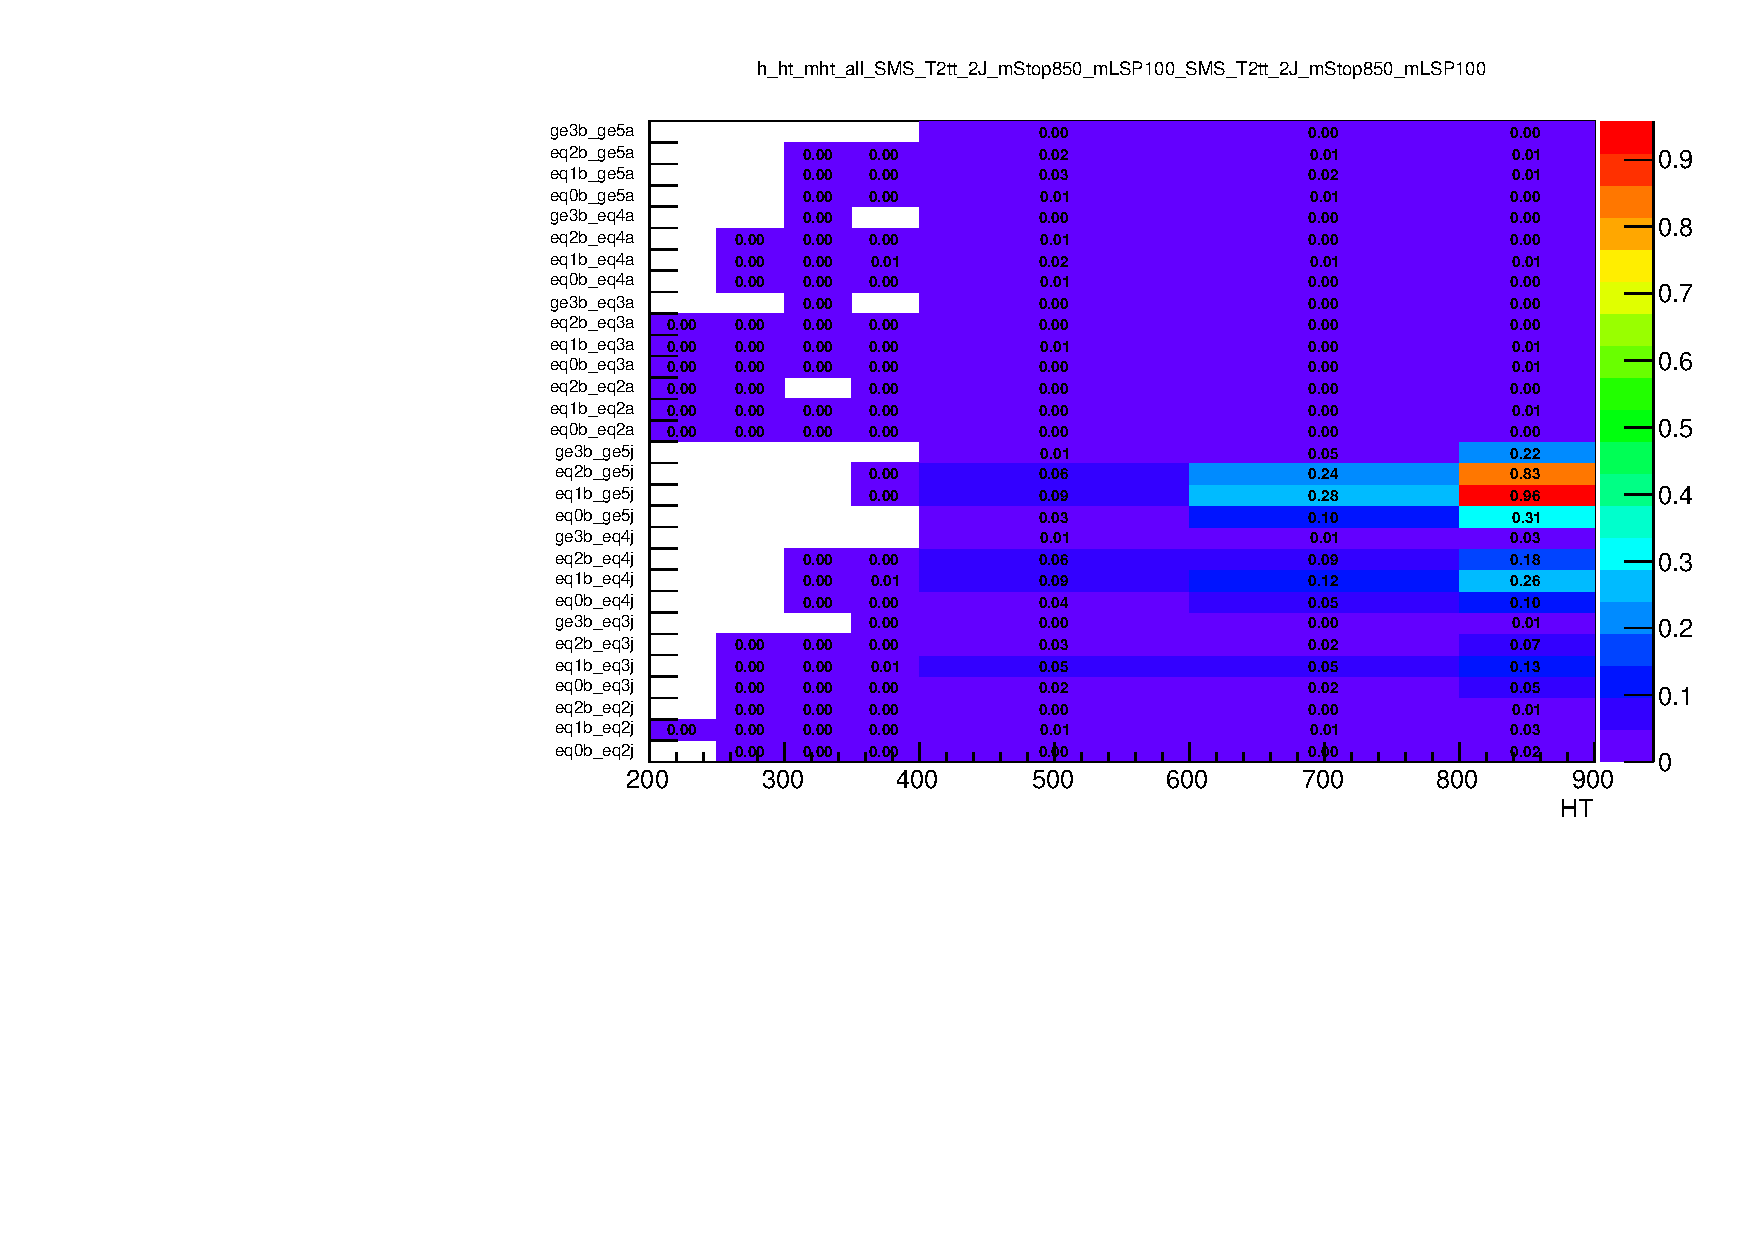
\includegraphics[width=0.5\textwidth]{figures/sensitivityStudy/h_ht_mht_all_SMS_T2tt_2J_mStop850_mLSP100}
    } 
    \subfigure[Expected counts in the \mj control region]{
      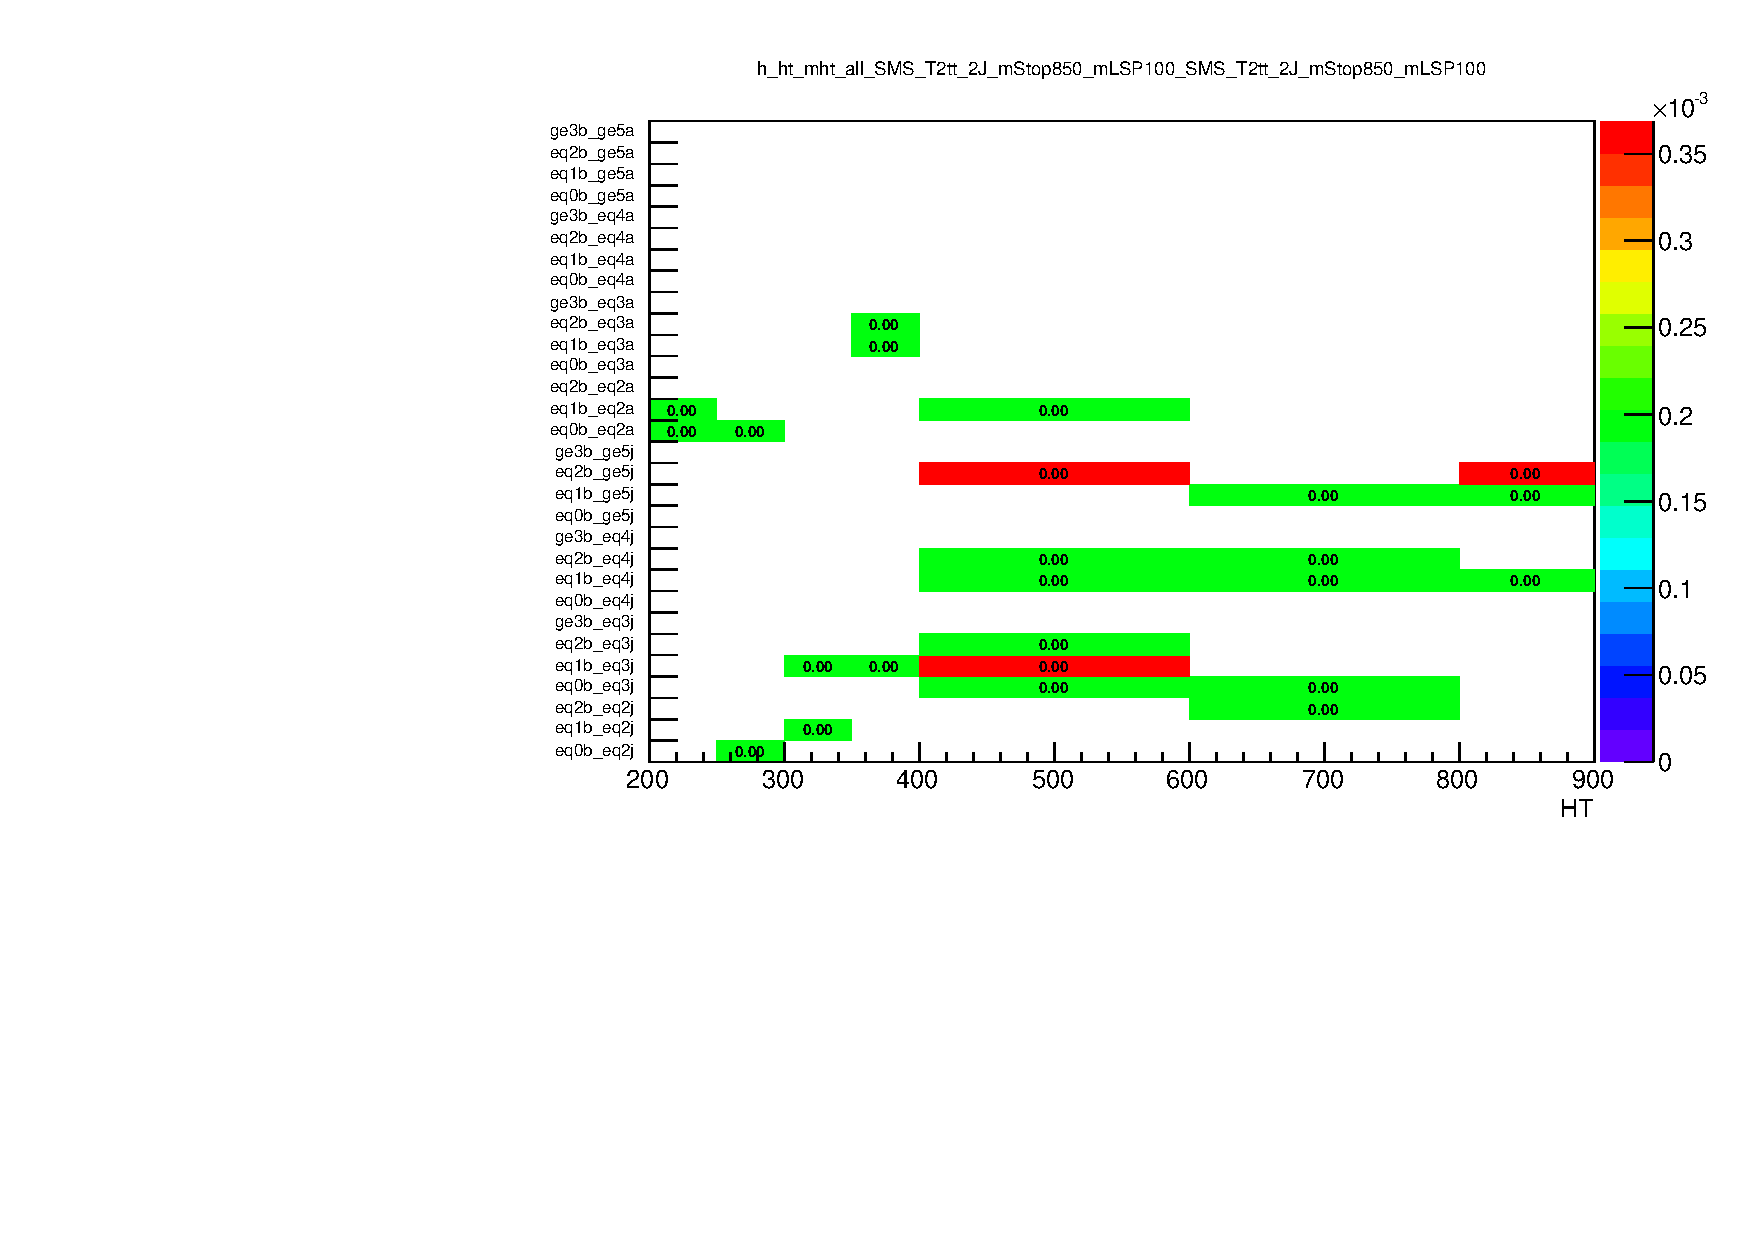
\includegraphics[width=0.5\textwidth]{figures/sensitivityStudy/m_ht_mht_all_SMS_T2tt_2J_mStop850_mLSP100}
    } \\
    \subfigure[Ratio of signal acceptance (\mj control region w.r.t. signal region)]{
      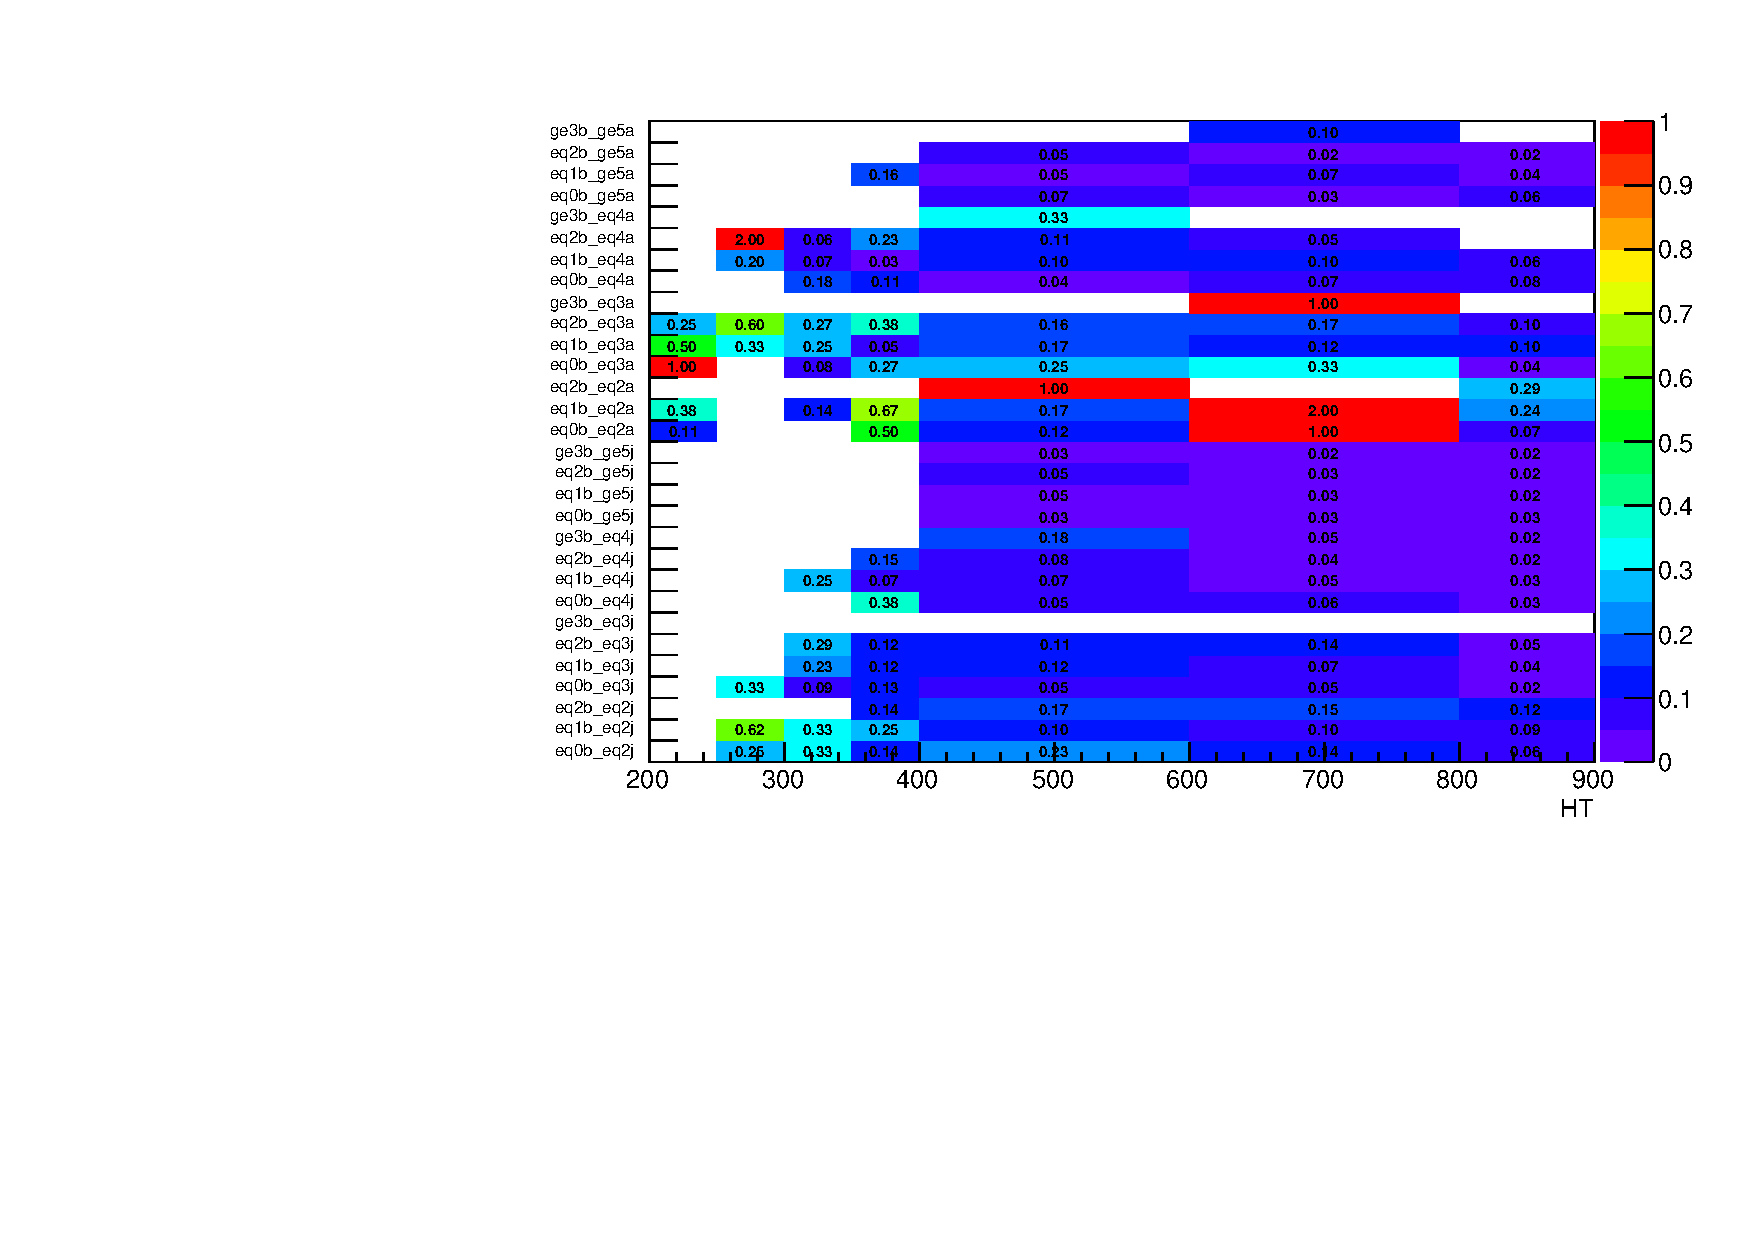
\includegraphics[width=0.5\textwidth]{figures/sensitivityStudy/relEff_singlemu_SMS_T2tt_2J_mStop850_mLSP100}
    }
    \subfigure[Ratio of S/B values (signal region w.r.t. \mj)]{
      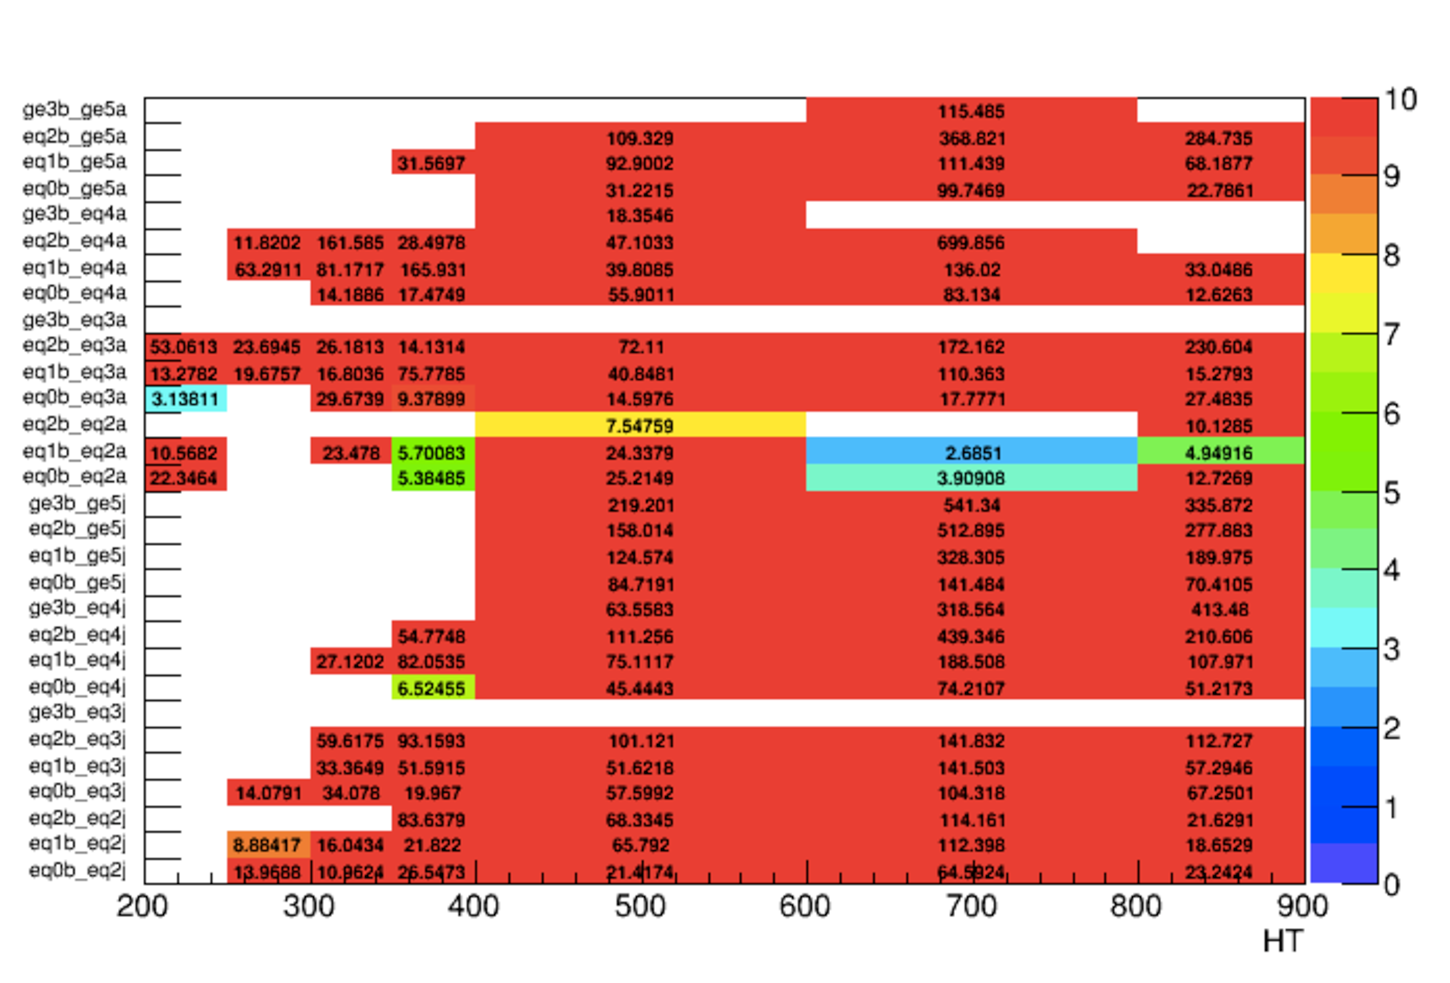
\includegraphics[width=0.5\textwidth]{figures/sensitivityStudy/doubleRatio_singlemu_SMS_T2tt_2J_mStop850_mLSP100}
    }
    \caption{Characterisation of signal acceptance and contamination
      in the signal and \mj control regions, respectively, for the
      benchmark model \texttt{T2tt} (850,100).}
    \label{fig:contamination}
  \end{center}
\end{figure}

Figure~\ref{fig:contamination} (c) shows the ratio of these expected
yields (signal region with respect to the \mj control region). The
ratio is typically small, at the percent level for the most sensitive
categories (\ie with four or more jets and one or two b-tagged jets).

In addition, the event counts from SM background processes in the \mj
control sample are significantly higher than in the signal region, as
no \alphat requirement is made for the \mj sample. Therefore, the S/B
ratios for the signal region relative to the \mj sample are larger by
many factors, typically $\gg$10. Figure~\ref{fig:contamination} (d)
shows the ratio of S/B$_{\rm signal}$ over S/B$_{\rm \mj}$ as a
function of the event category and \scalht bin.

Figure~\ref{fig:contamination_t1tttt} characterises the level of
signal contamination in the \mj control sample for the benchmark model
\texttt{T1tttt} ($m_{Gluino}=1500$ GeV, $m_{LSP}=100$ GeV). A larger level of contamination is
expected for this model (with respect to \texttt{T2tt}), due to the
presence of four W bosons produced in the decay of the gluino-pair
system (via off-shell top squarks). The ratio of yields in the signal
and \mj control regions is at the level of $\sim$10--20\% for the most
sensitive categories (\ie with four or more jets, two or more b-tagged
jets, and at high \scalht). The ratio of S/B values for the signal
region relative to the \mj sample is still large, typically $\gg$10.

\begin{figure}[h!]
  \begin{center}
    \subfigure[Expected counts in the signal region]{
      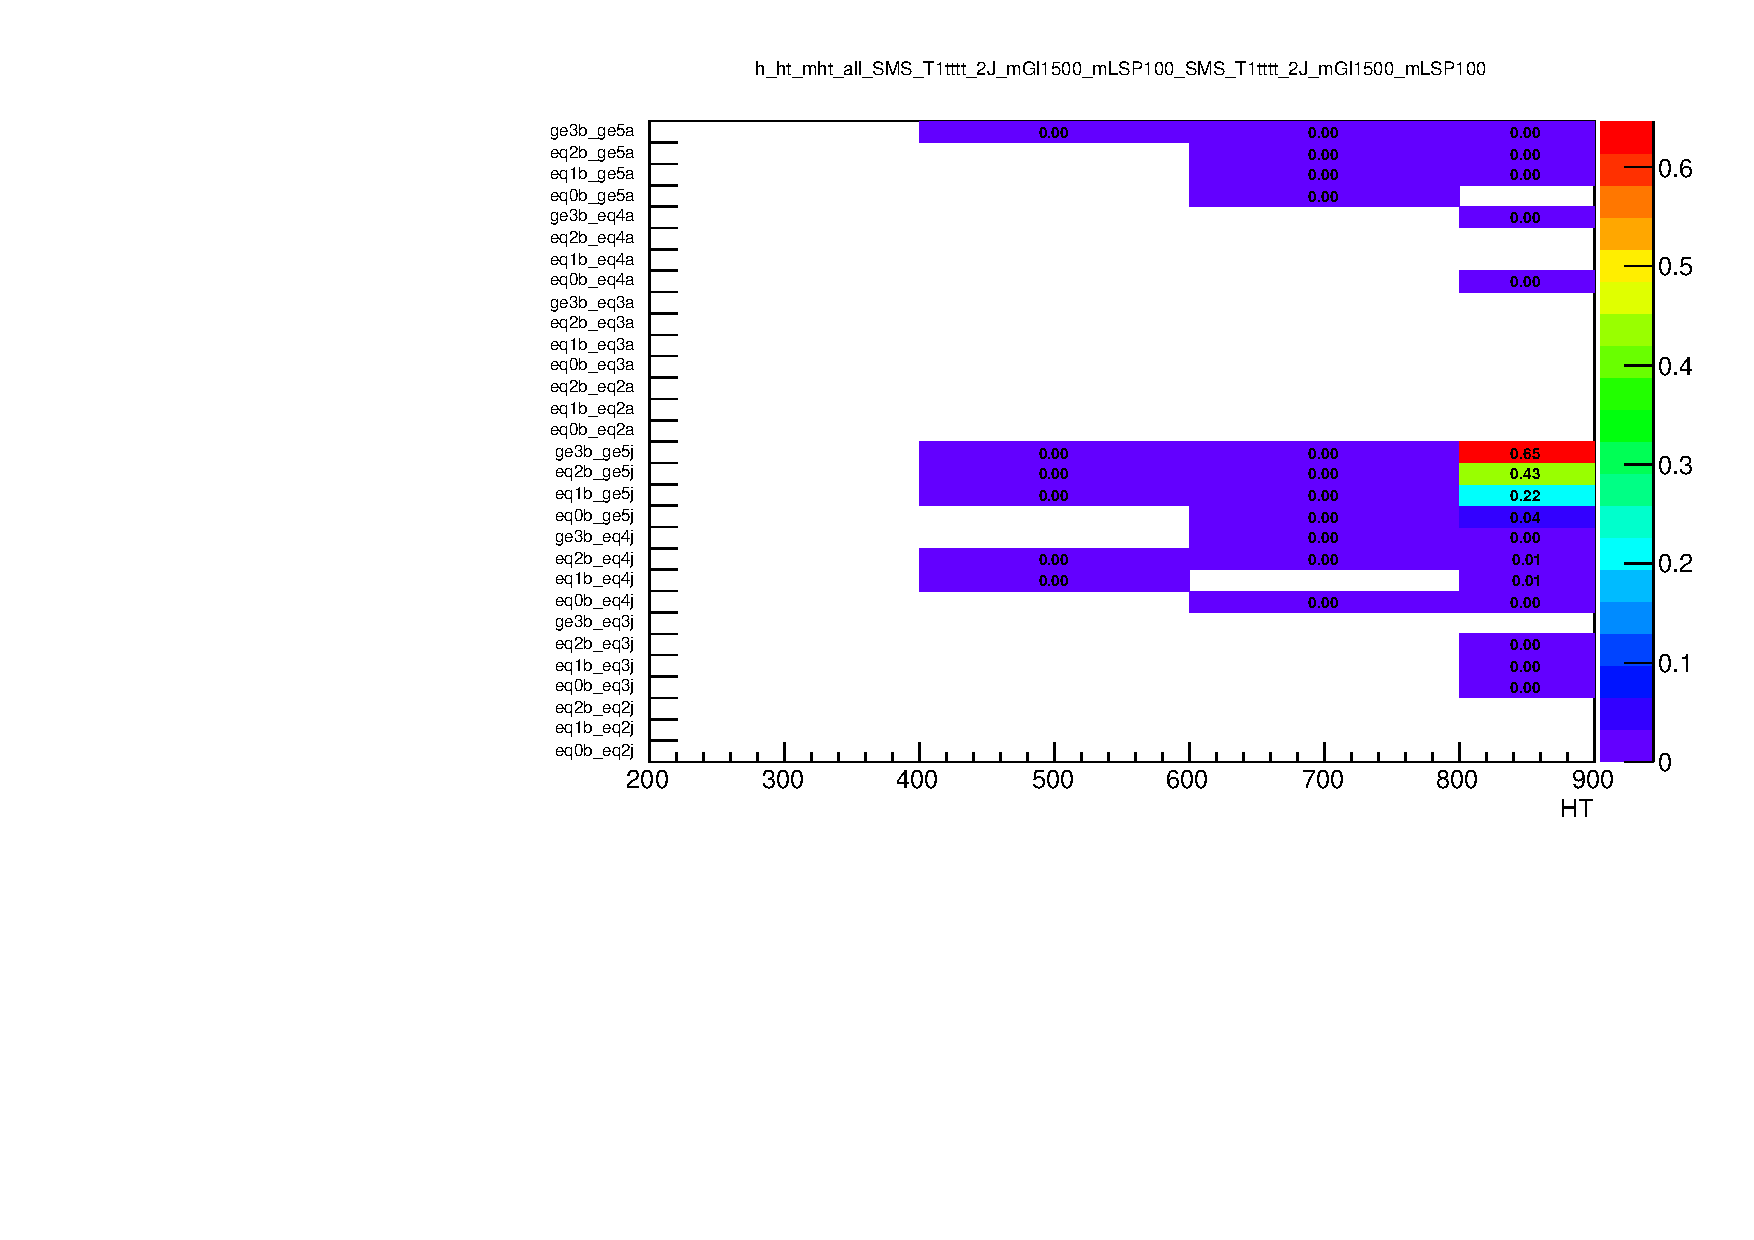
\includegraphics[width=0.5\textwidth]{figures/sensitivityStudy/h_ht_mht_all_SMS_T1tttt_2J_mGl1500_mLSP100}
    } 
    \subfigure[Expected counts in the \mj control region]{
      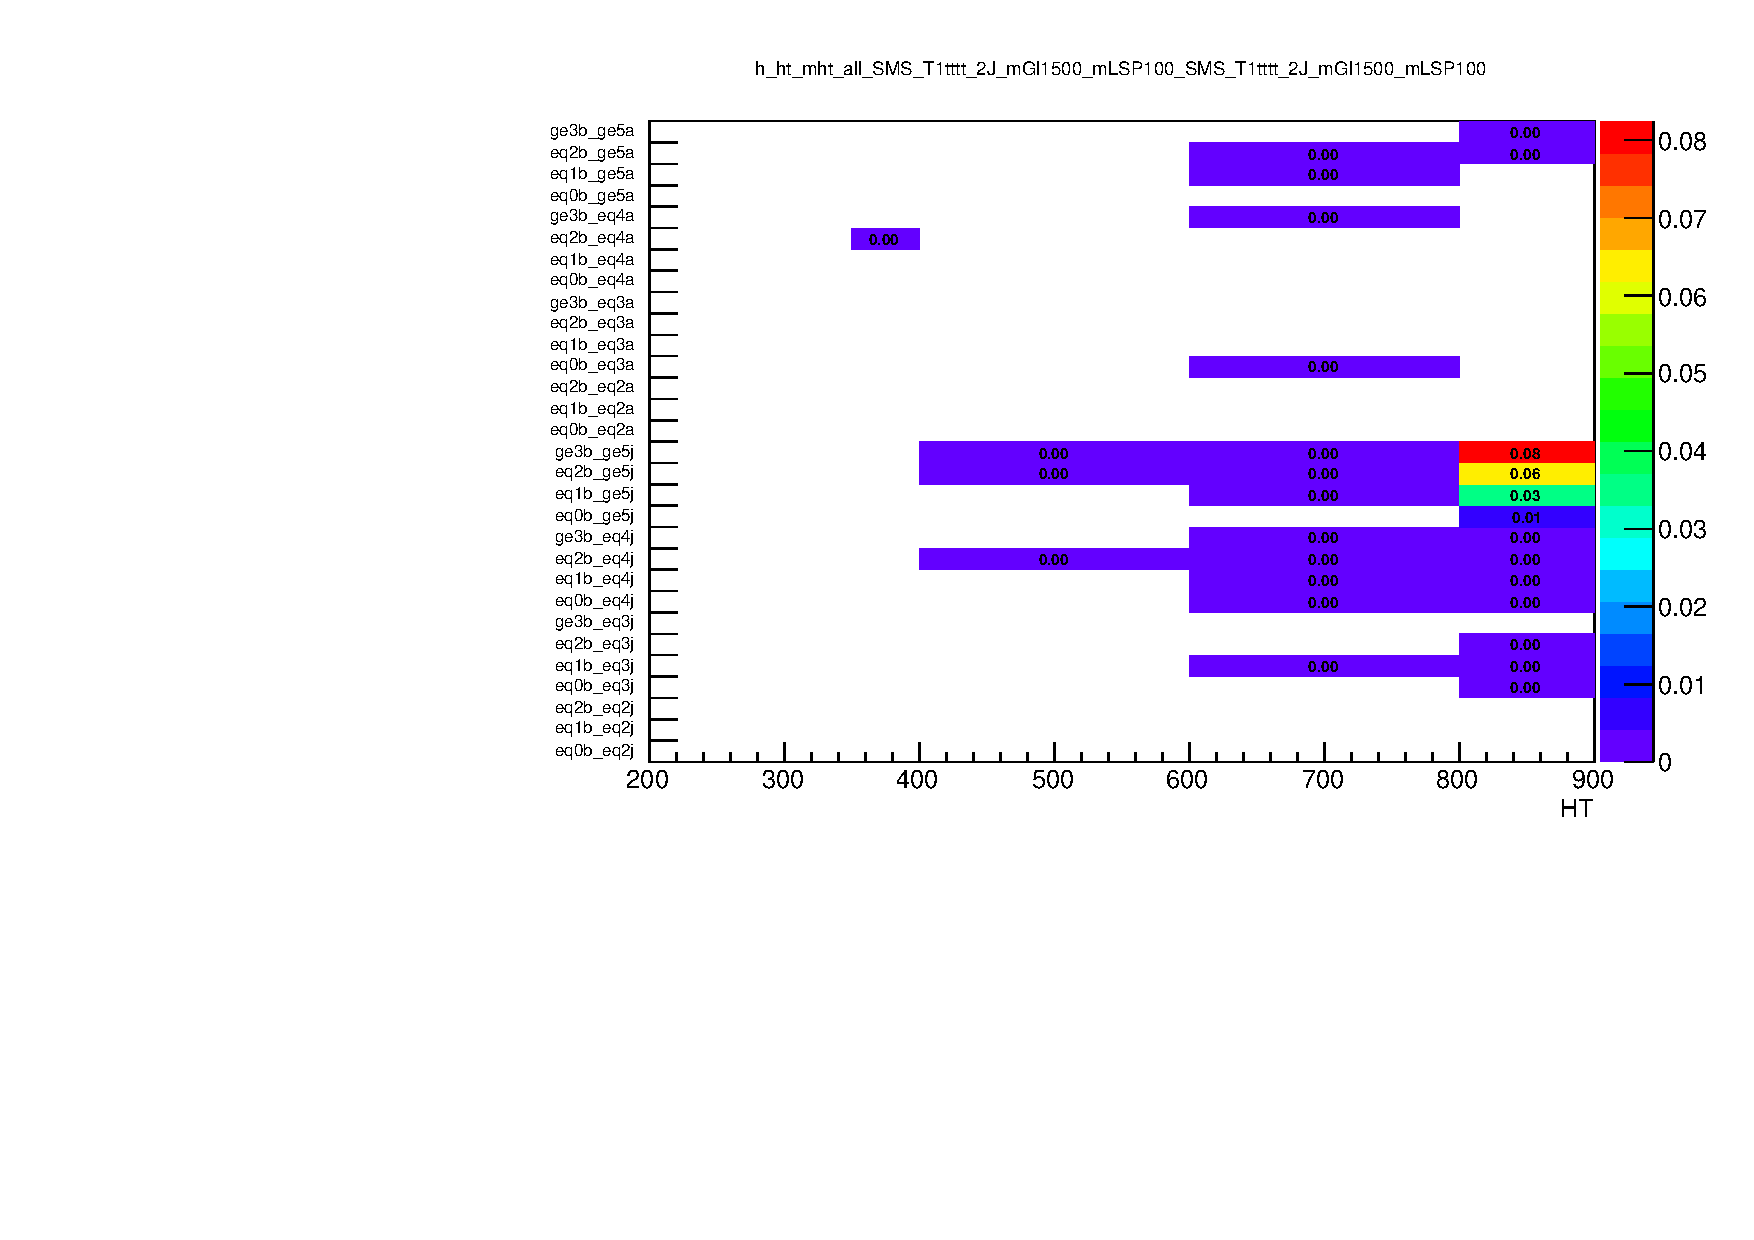
\includegraphics[width=0.5\textwidth]{figures/sensitivityStudy/m_ht_mht_all_SMS_T1tttt_2J_mGl1500_mLSP100}
    } \\
    \subfigure[Ratio of signal acceptance (signal region w.r.t. \mj)]{
      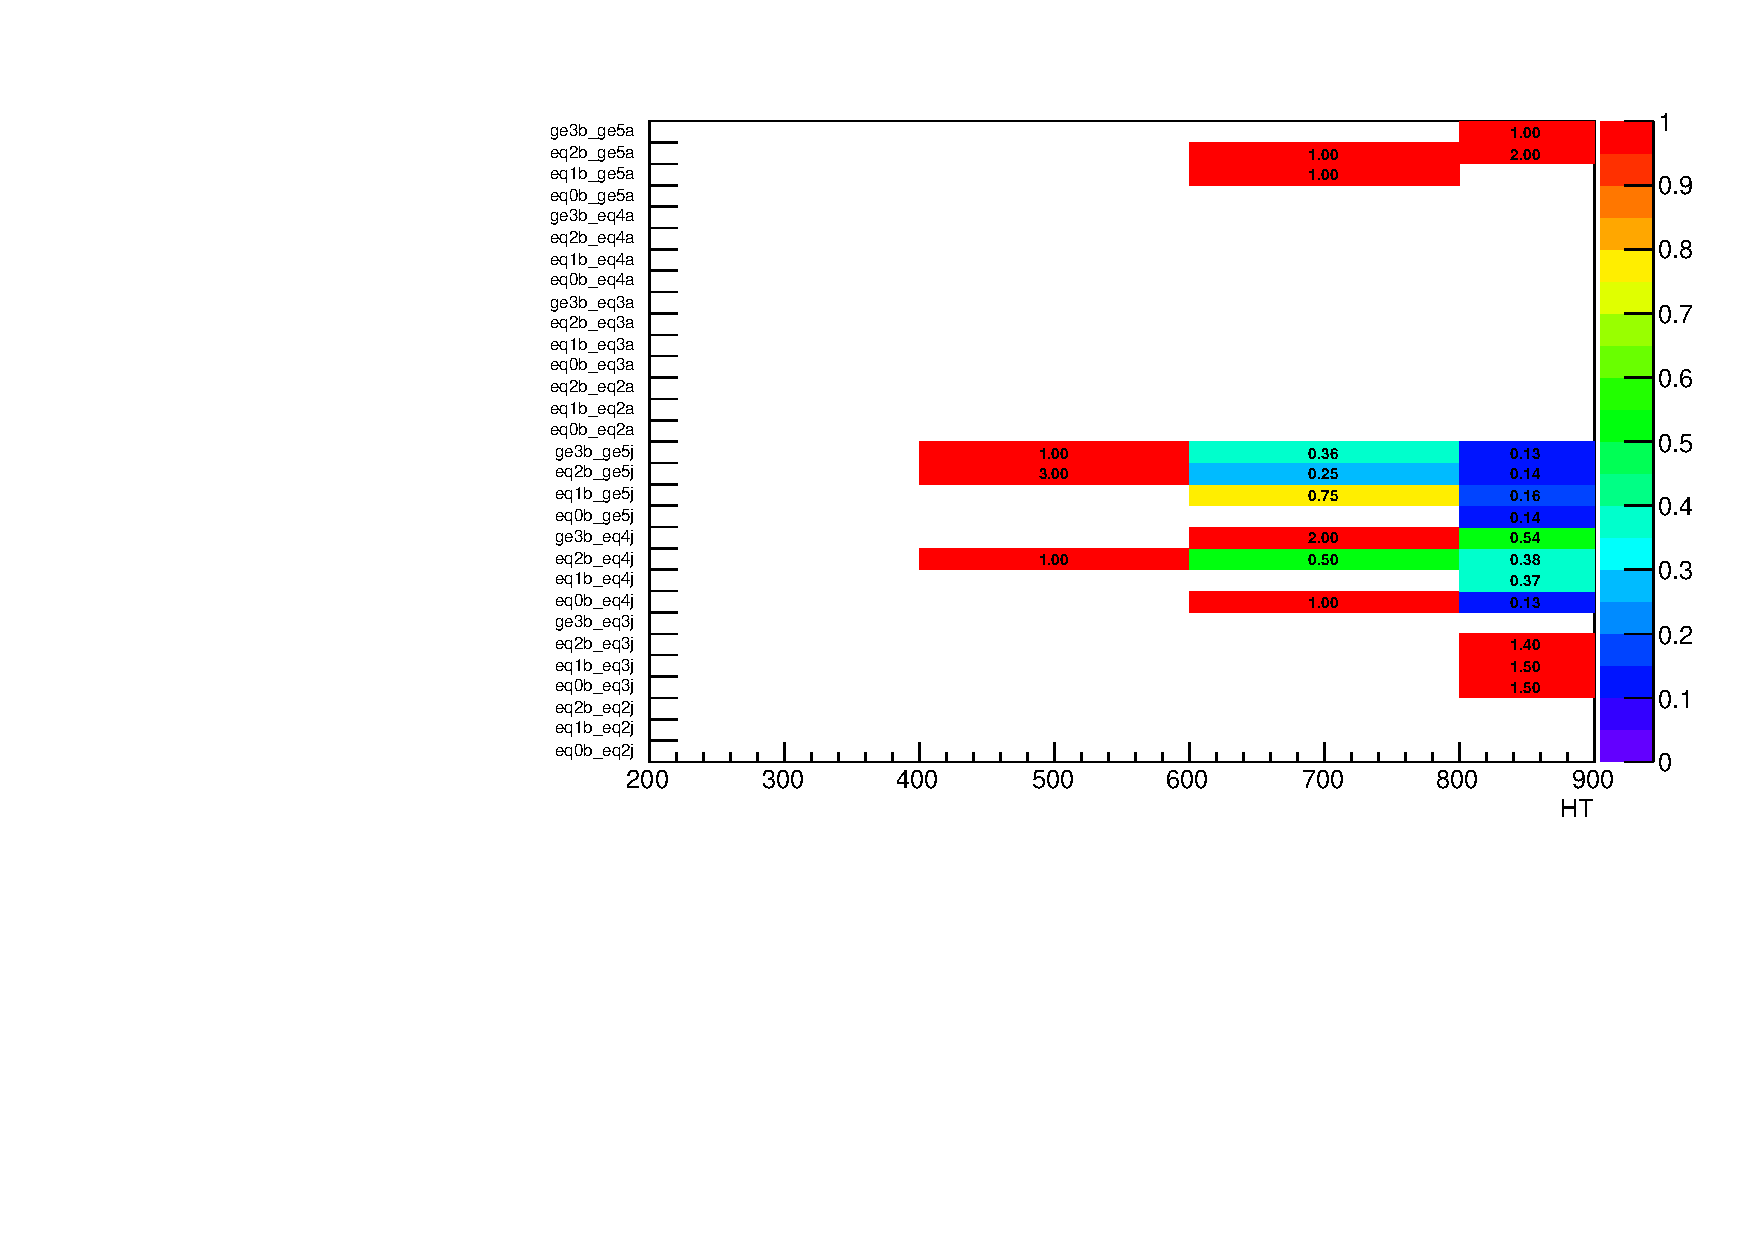
\includegraphics[width=0.5\textwidth]{figures/sensitivityStudy/relEff_singlemu_SMS_T1tttt_2J_mGl1500_mLSP100}
    }
    \subfigure[Ratio of S/B values (signal region w.r.t. \mj)]{
      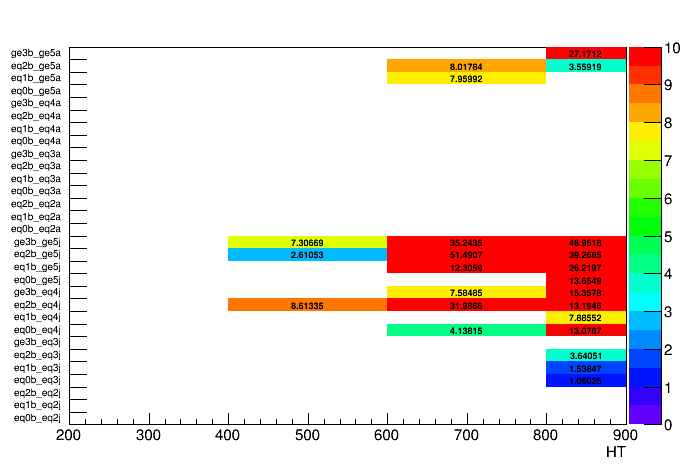
\includegraphics[width=0.5\textwidth]{figures/sensitivityStudy/doubleRatio_singlemu_SMS_T1tttt_2J_mGl1500_mLSP100}
    }
    \caption{Characterisation of signal acceptance and contamination
      in the signal and \mj control regions, respectively, for the
      benchmark model \texttt{T1tttt} (1500,100).}
    \label{fig:contamination_t1tttt}
  \end{center}
\end{figure}

For both models (and in general), the level of contamination for the
\mmj sample is smaller still due to the requirement of a second
muon. The contamination for the \gj sample is expected to be zero for
the models under consideration. 

Finally, the potential for signal contamination in all control samples
is fully accounted for in the likelihood model used to extract
information on sensitivity to any given signal model.

\subsection{Systematic uncertainties on signal efficiency times acceptance}
\label{sec:sig-syst}

For these results the same systematic uncertainty on the signal yield 
as in the previous Run 1 analysis is assumed \cite{CMS_AN_2013-366}. 
The following sources of uncertainty were considered: 
luminosity, parton distribution
functions, jet energy scale, initial state radiation, 
efficiencies of the \mht/\met filter and ``dead ECAL'' filter. 
Each contribution is considered to be independent and all contributions are
summed in quadrature. \\
The uncertainty applied is 30\% for all the mass point in the vicinity of the ``diagonal'', i.e. where $m_{Gluino}-m_{LSP}<m_{top}$, 
and 15\% for all the other points. 
The systematic is taken as fully correlated across all the bins (see Sec.~\ref{sec:likelihood}). 
The uncorrelated approach has been checked to give very similar results. \\
No uncertainty for the signal \MHT template is considered in these results, 
but dedicated studies will be carried on in the future about this.


\subsection{Expected exclusion limits and discovery significance}
\label{subsec:susy_results}

In order to extract the signal contribution in the fit, the distribution of events according to the \mht variable, 
encoded as template histograms, is used as described in Sec.~\ref{sec:had-shape} and \ref{sec:likelihood}. \\
Upper limits on the cross section and discovery significance are computed using the asymptotic formulae and the pre-fit Asimov datasets \cite{AsymptoticFormulae}. 
The upper limits are computed using the $\text{CL}_{s}$ criterion \cite{CLsTechnique}. \\
All the statistical results are produced using the \textit{combine} tool, 
provided within the HiggsAnalysis-CombinedLimit package \cite{Combine}. 

%Due to CPU constraints, only a subset of event categories (but all \scalht bins
%within a category) are considered to extract the final result. 
%The categories entering the final fit are chosen based as the 10 most sensitive ones according to the expected discovery significance.

In Figure ~\ref{fig:T1bbbb_plane_xs} and ~\ref{fig:T1bbbb_plane_mu} the expected upper limits on the cross section and the signal strength $\mu=\sigma/\sigma_{\mathrm{theory}}$ are shown for 1.26 \ifb of integrated luminosity, in the $(m_{Gluino},m_{LSP})$ plane, for the \texttt{T1bbbb} model. 
The exclusion contour is also shown together with $\pm1\sigma$ uncertainty (dashed lines) from the expected limit. 

\begin{figure}
  \caption{95\% C.L. expected (solid black line) oberved (solid red line) upper limit on the cross section for the \texttt{T1bbbb} model.\label{fig:T1bbbb_plane_xs}}
  \begin{center}
    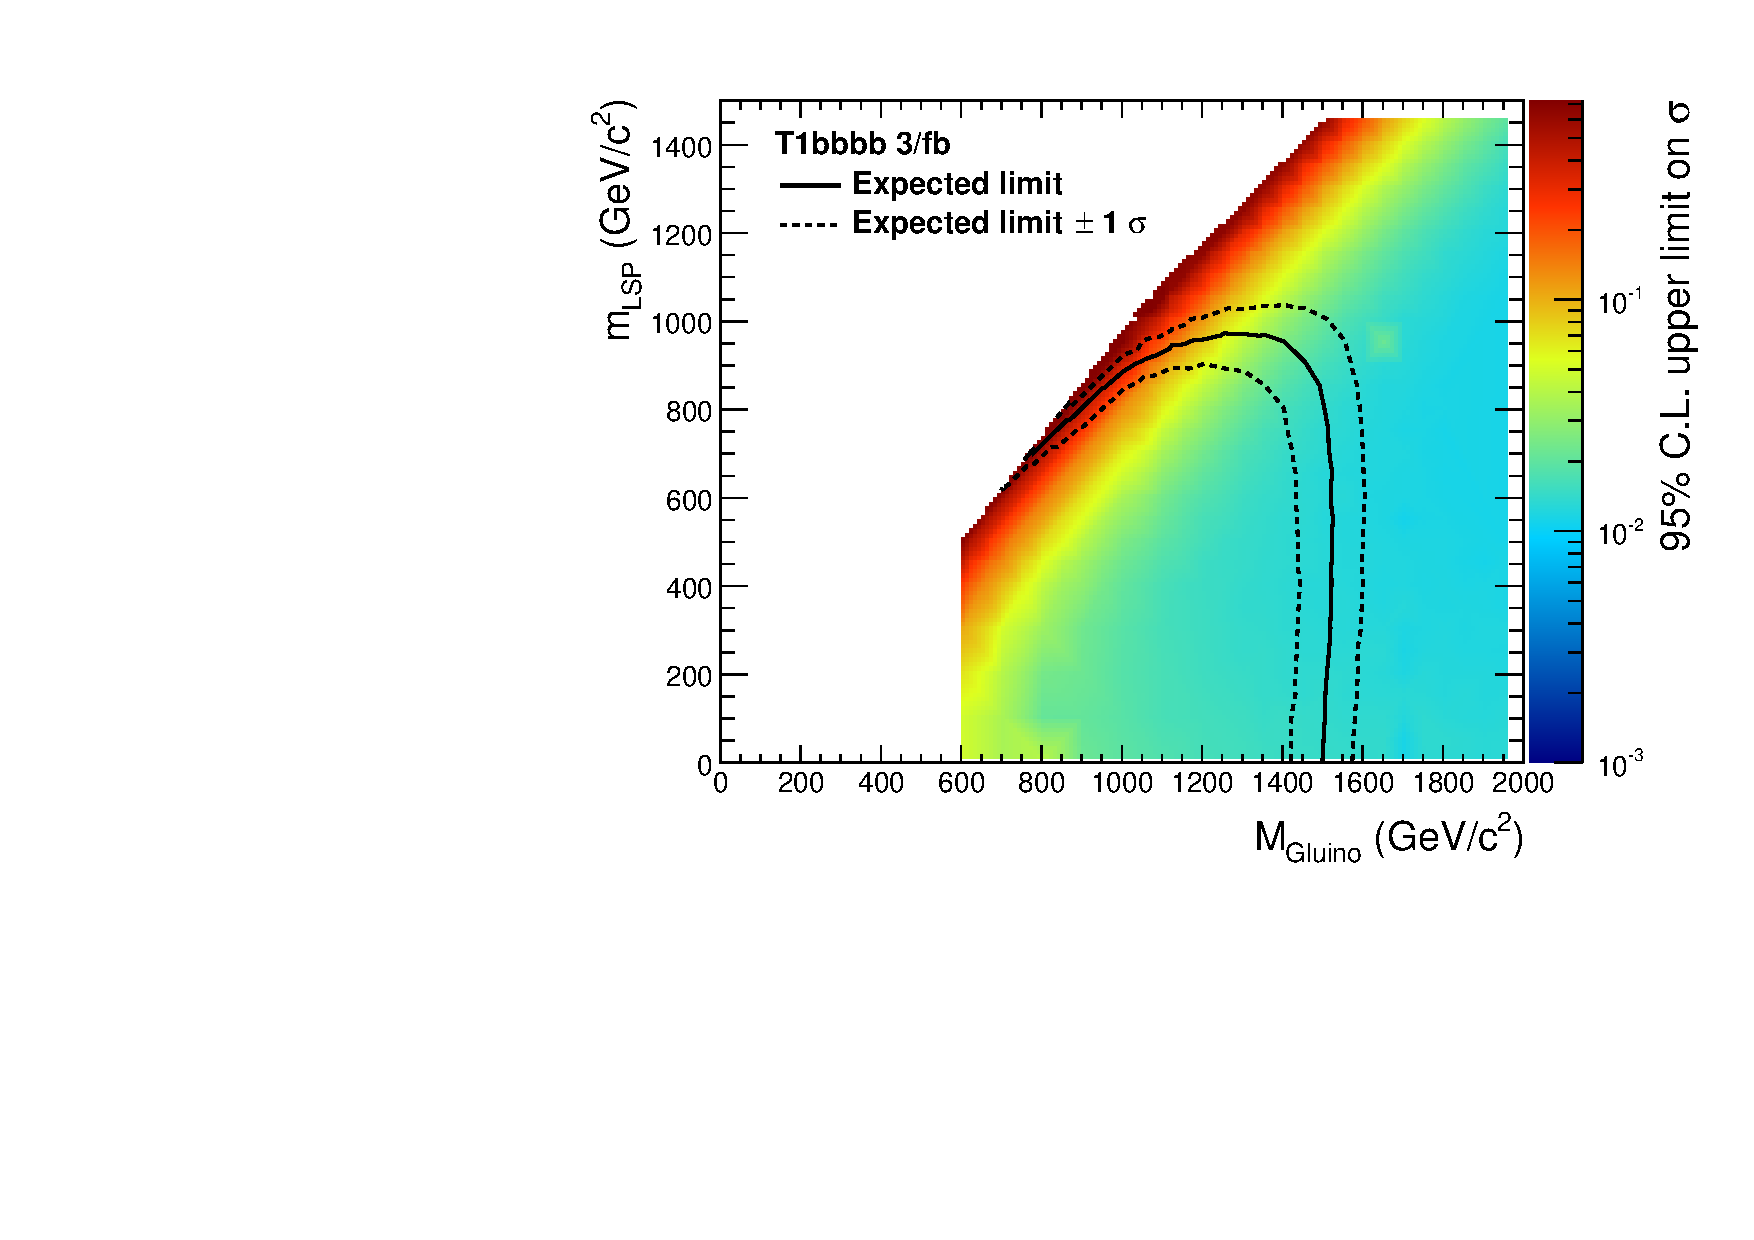
\includegraphics[width=0.5\textwidth]{figures/susyResults/xs_contour_withHisto}
  \end{center}
\end{figure}

\begin{figure}
  \caption{95\% C.L. expected (solid black line) oberved (solid red line) upper limit on the signal strength for the \texttt{T1bbbb} model.\label{fig:T1bbbb_plane_mu}}
  \begin{center}
    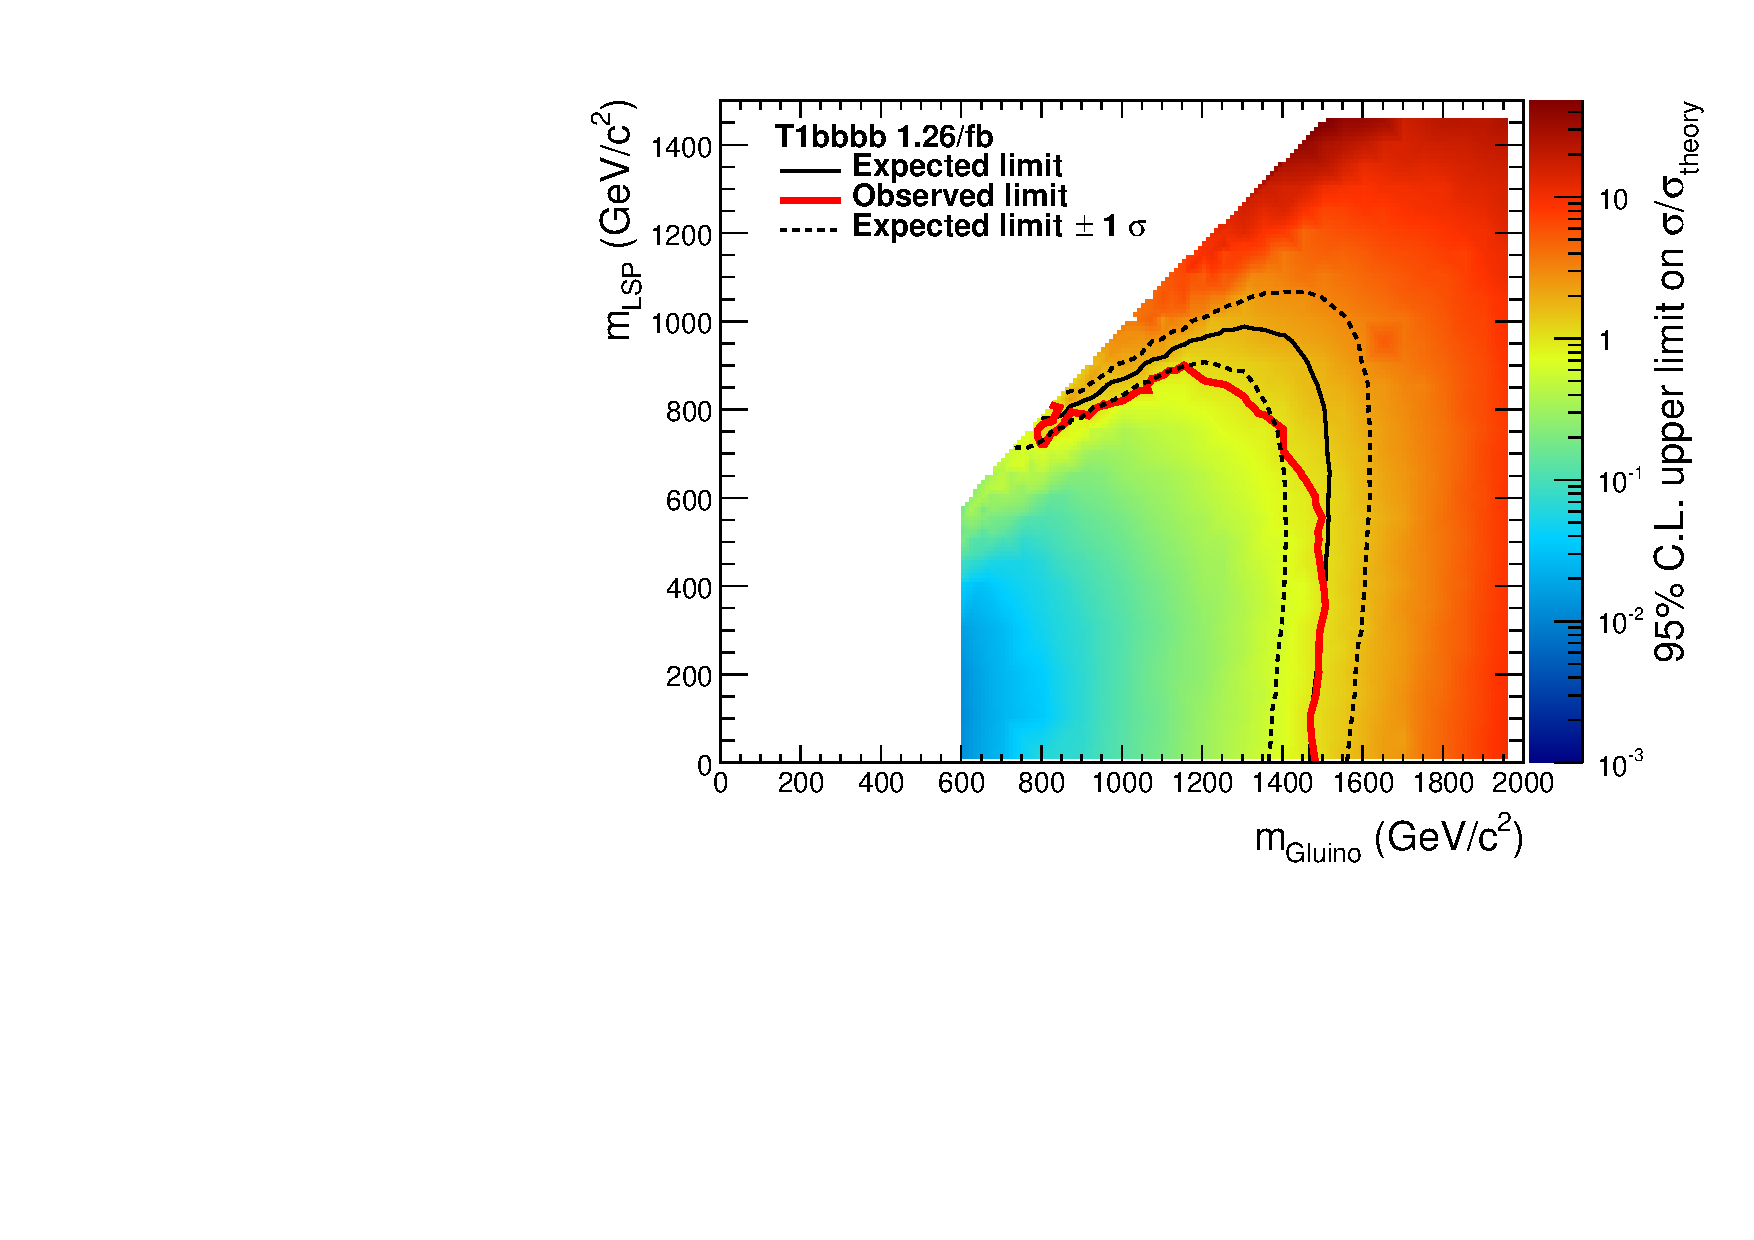
\includegraphics[width=0.5\textwidth]{figures/susyResults/mu_contour_withHisto}
  \end{center}
\end{figure}


% FIXME: this needs update
%% The \mht templates histograms for the backgrounds together with some benchmark models are shown in Figs.~\ref{fig:mht_eq0b_eq4j},\ref{fig:mht_eq0b_ge5j},\ref{fig:mht_eq0b_ge5a},\ref{fig:mht_eq1b_ge5j},\ref{fig:mht_eq2b_ge5a},\ref{fig:mht_ge3b_ge5j} for the most relevant \HT bins. 

%% \begin{figure}
%%   \begin{center}
%%     \subfigure[$350 < \HT < 400  \gev$]{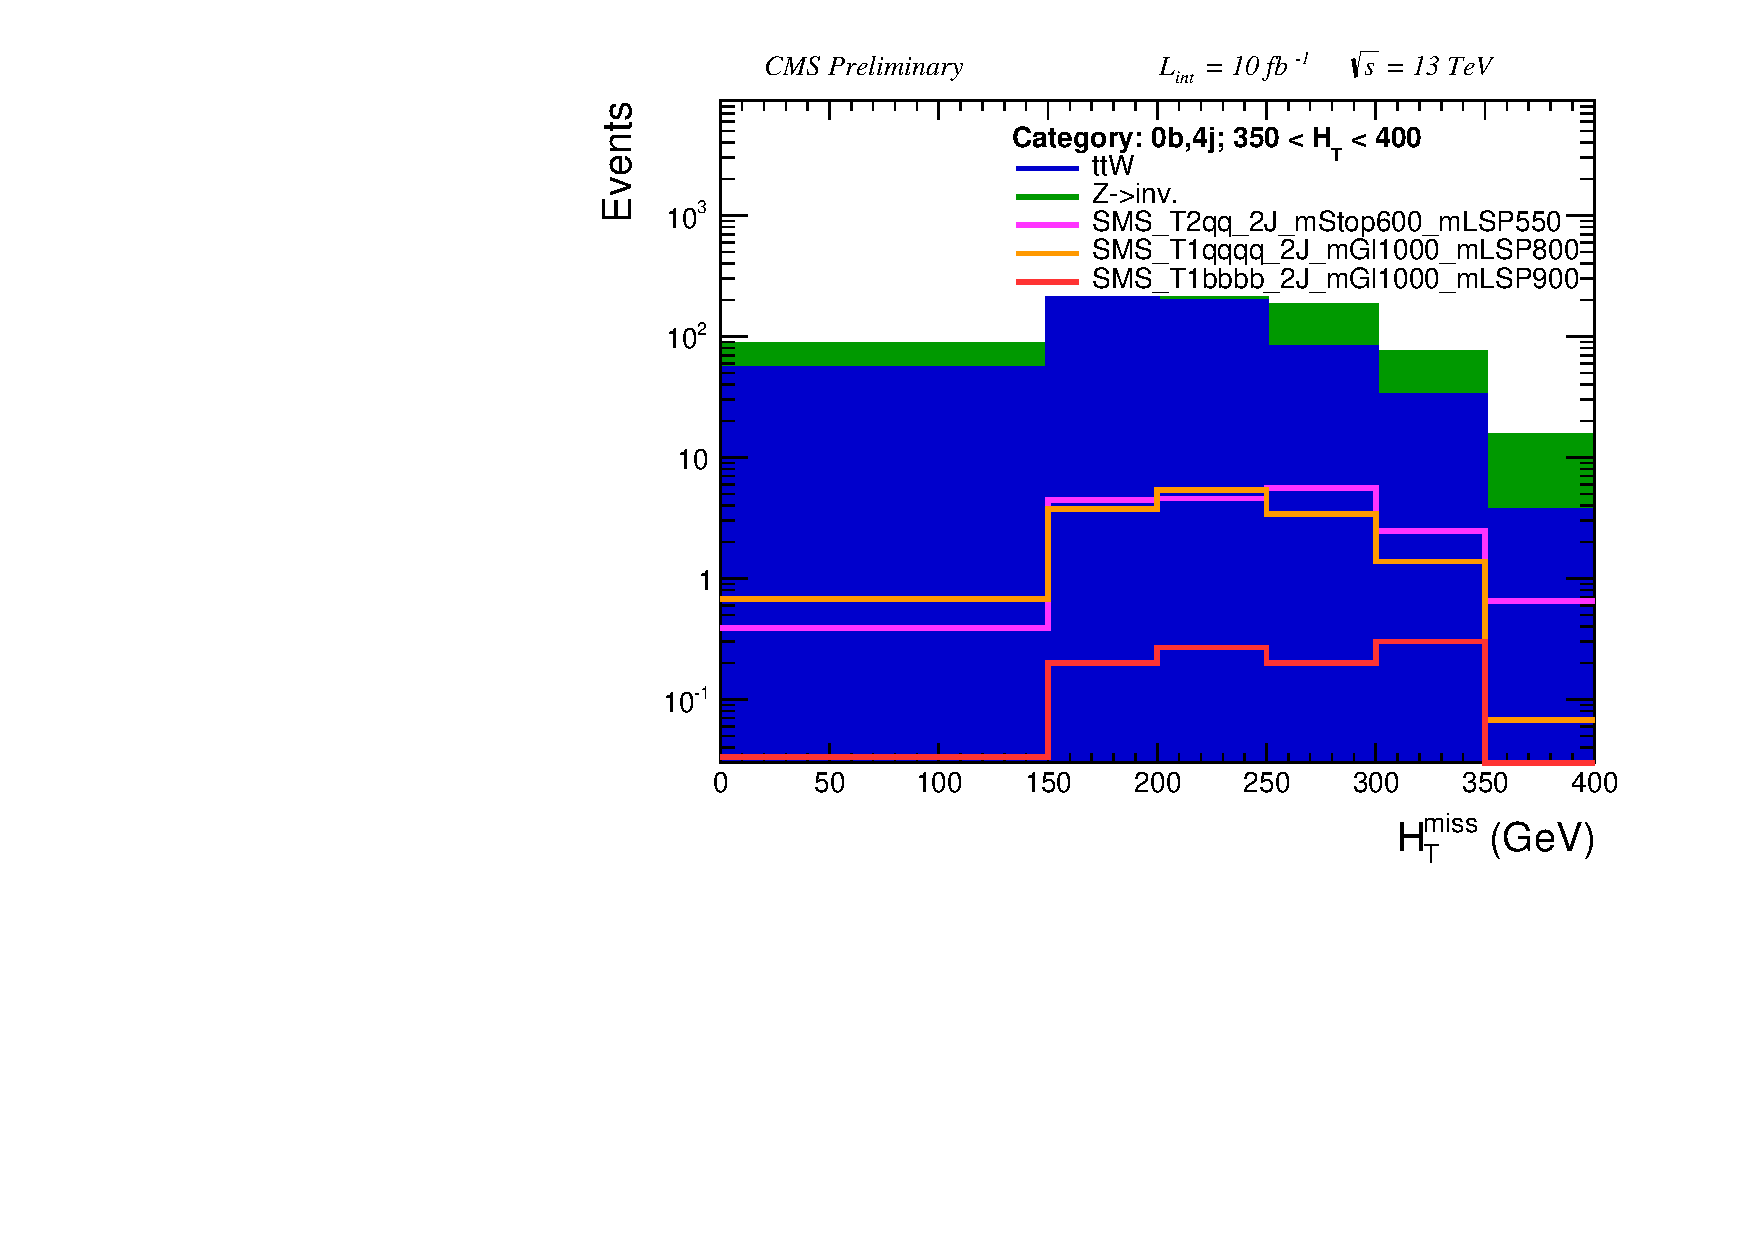
\includegraphics[width=0.5\textwidth]{figures/susyResults/MHT_eq0b_eq4j_350_400.pdf}} ~~
%%     \subfigure[$400 < \HT < 600  \gev$]{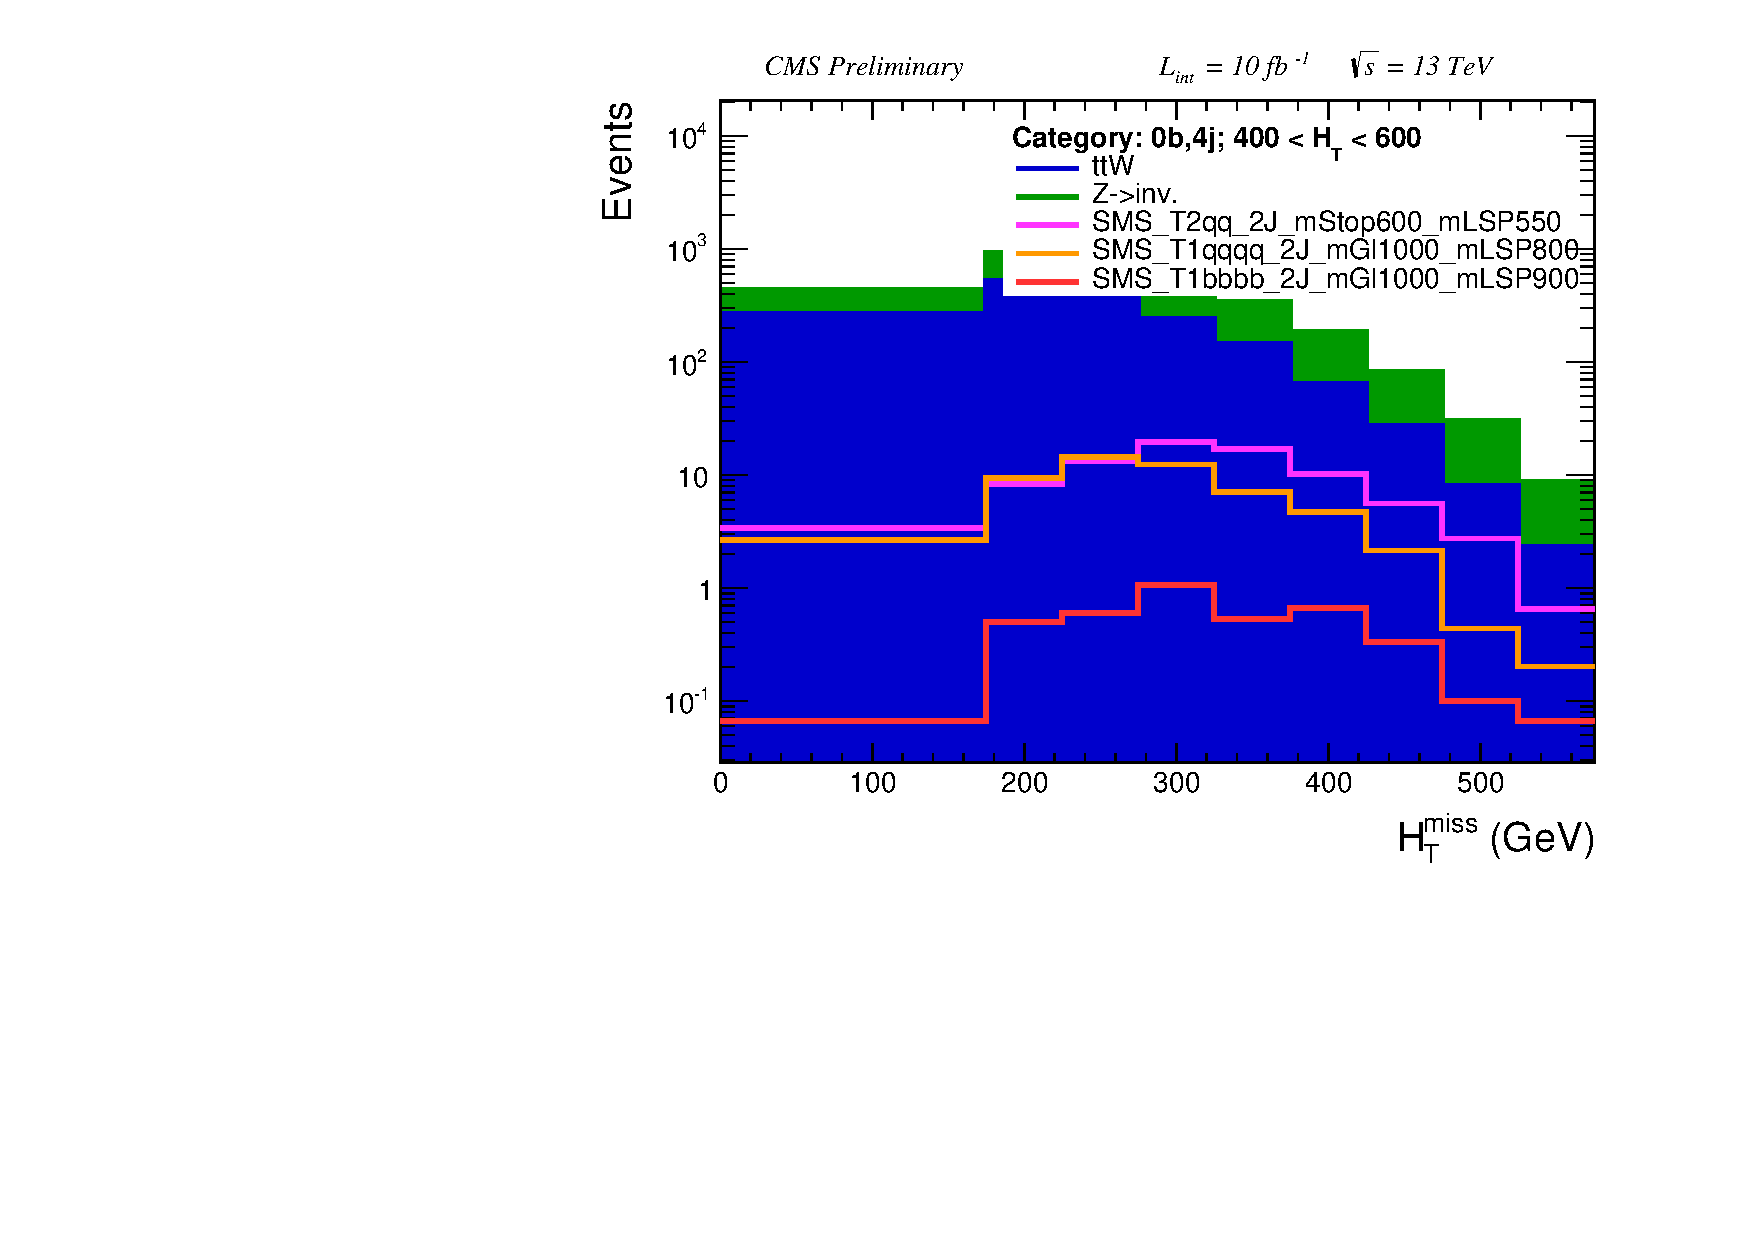
\includegraphics[width=0.5\textwidth]{figures/susyResults/MHT_eq0b_eq4j_400_600.pdf}} \\
%%     \subfigure[$600 < \HT < 800  \gev$]{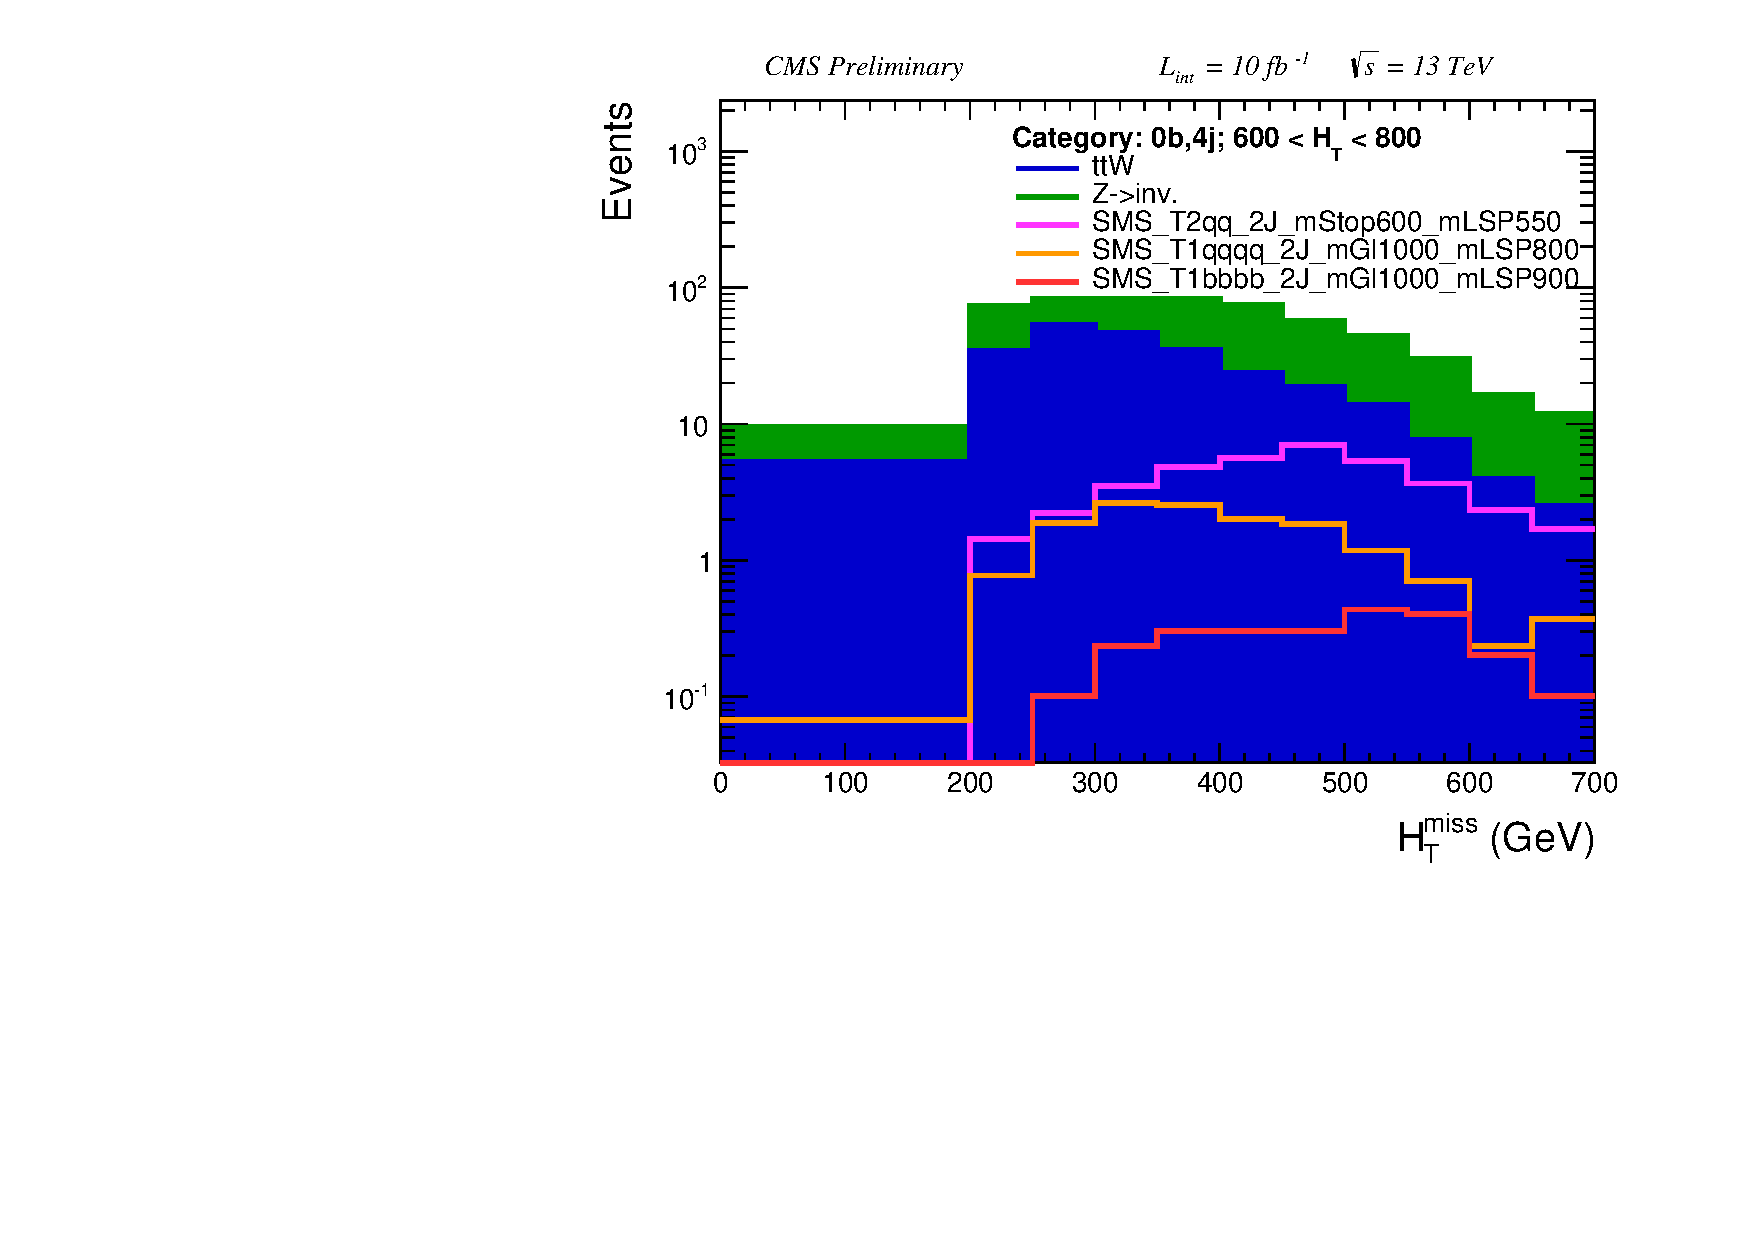
\includegraphics[width=0.5\textwidth]{figures/susyResults/MHT_eq0b_eq4j_600_800.pdf}} ~~
%%     \subfigure[$\HT > 800  \gev$]{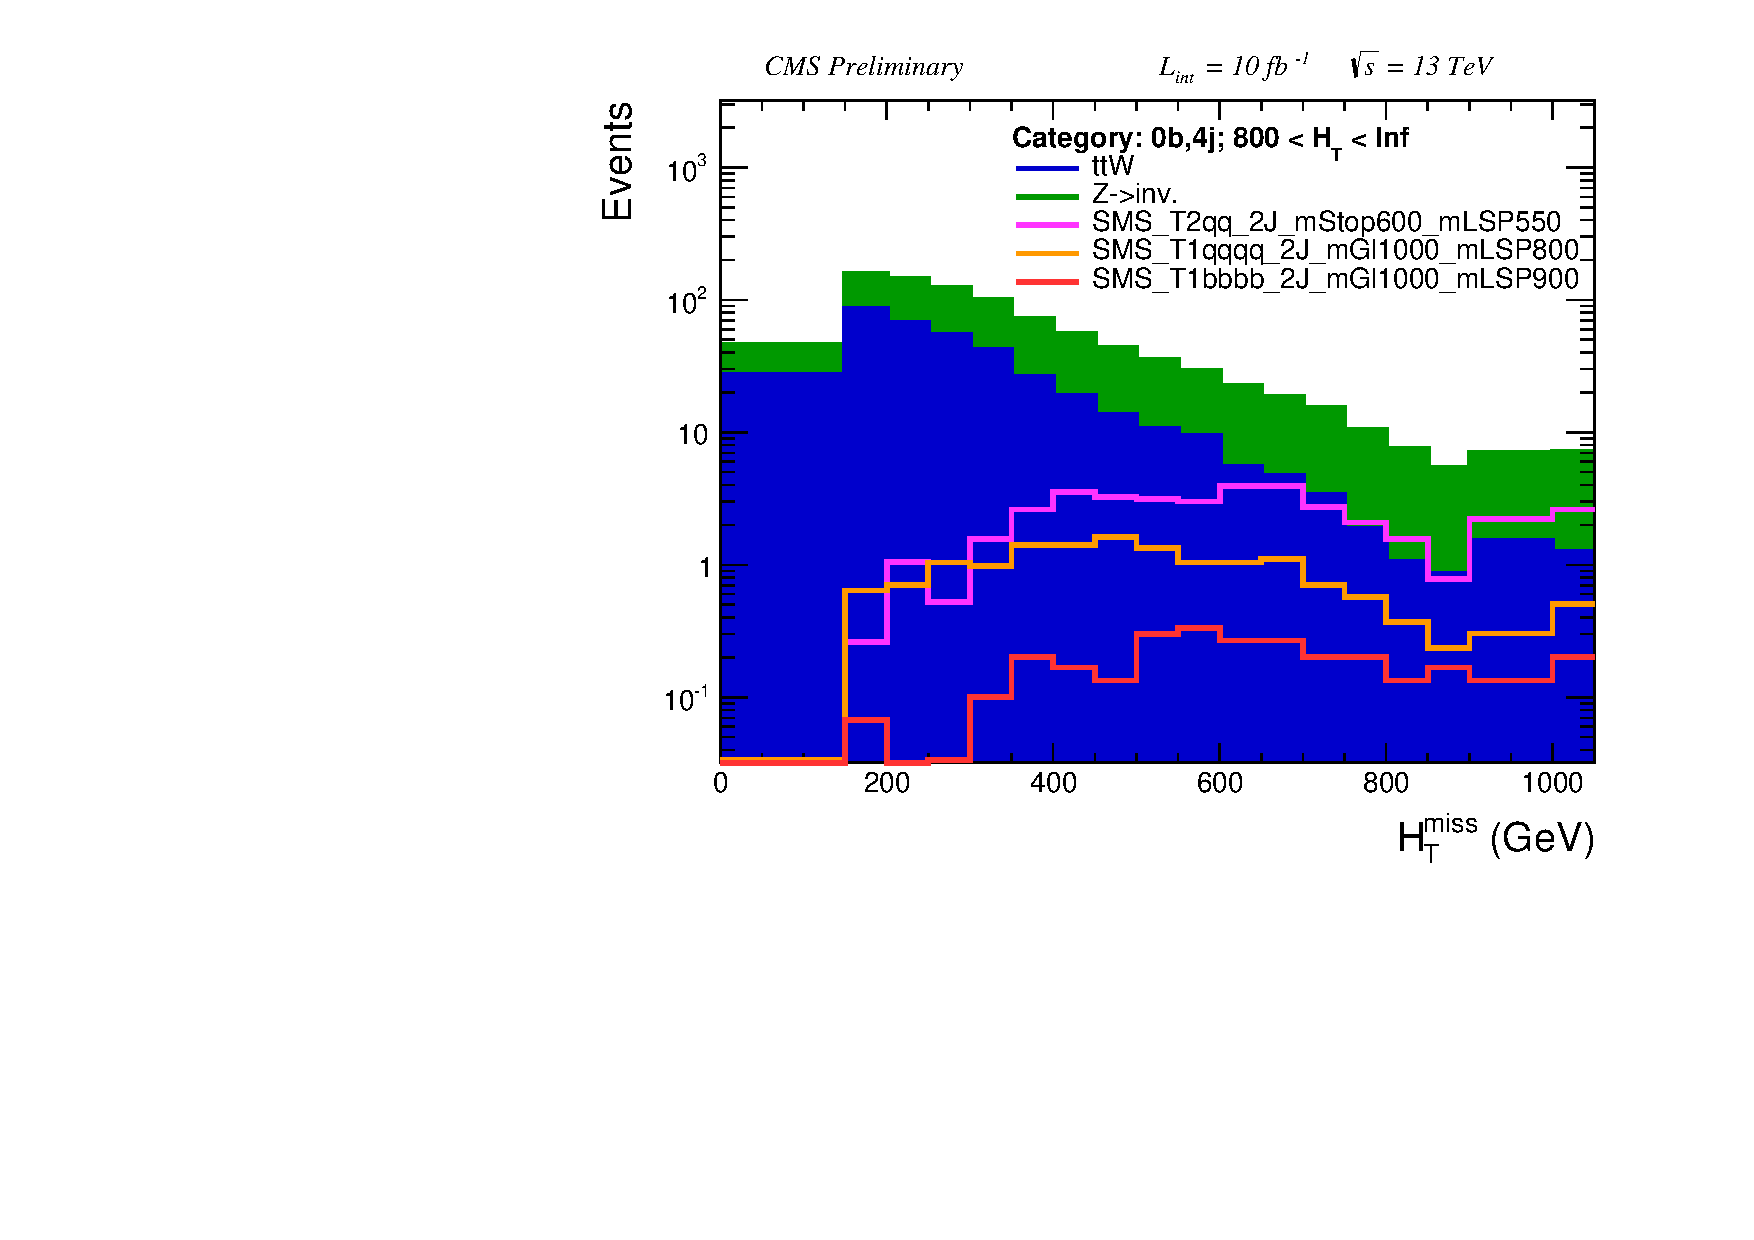
\includegraphics[width=0.5\textwidth]{figures/susyResults/MHT_eq0b_eq4j_800_Inf.pdf}} \\
%%     \caption{\mht templates for the $\njet=4$, $\nb=0$ category.}
%%     \label{fig:mht_eq0b_eq4j}
%%   \end{center}
%% \end{figure}


%% \begin{figure}
%%   \begin{center}
%%     \subfigure[$400 < \HT < 600  \gev$]{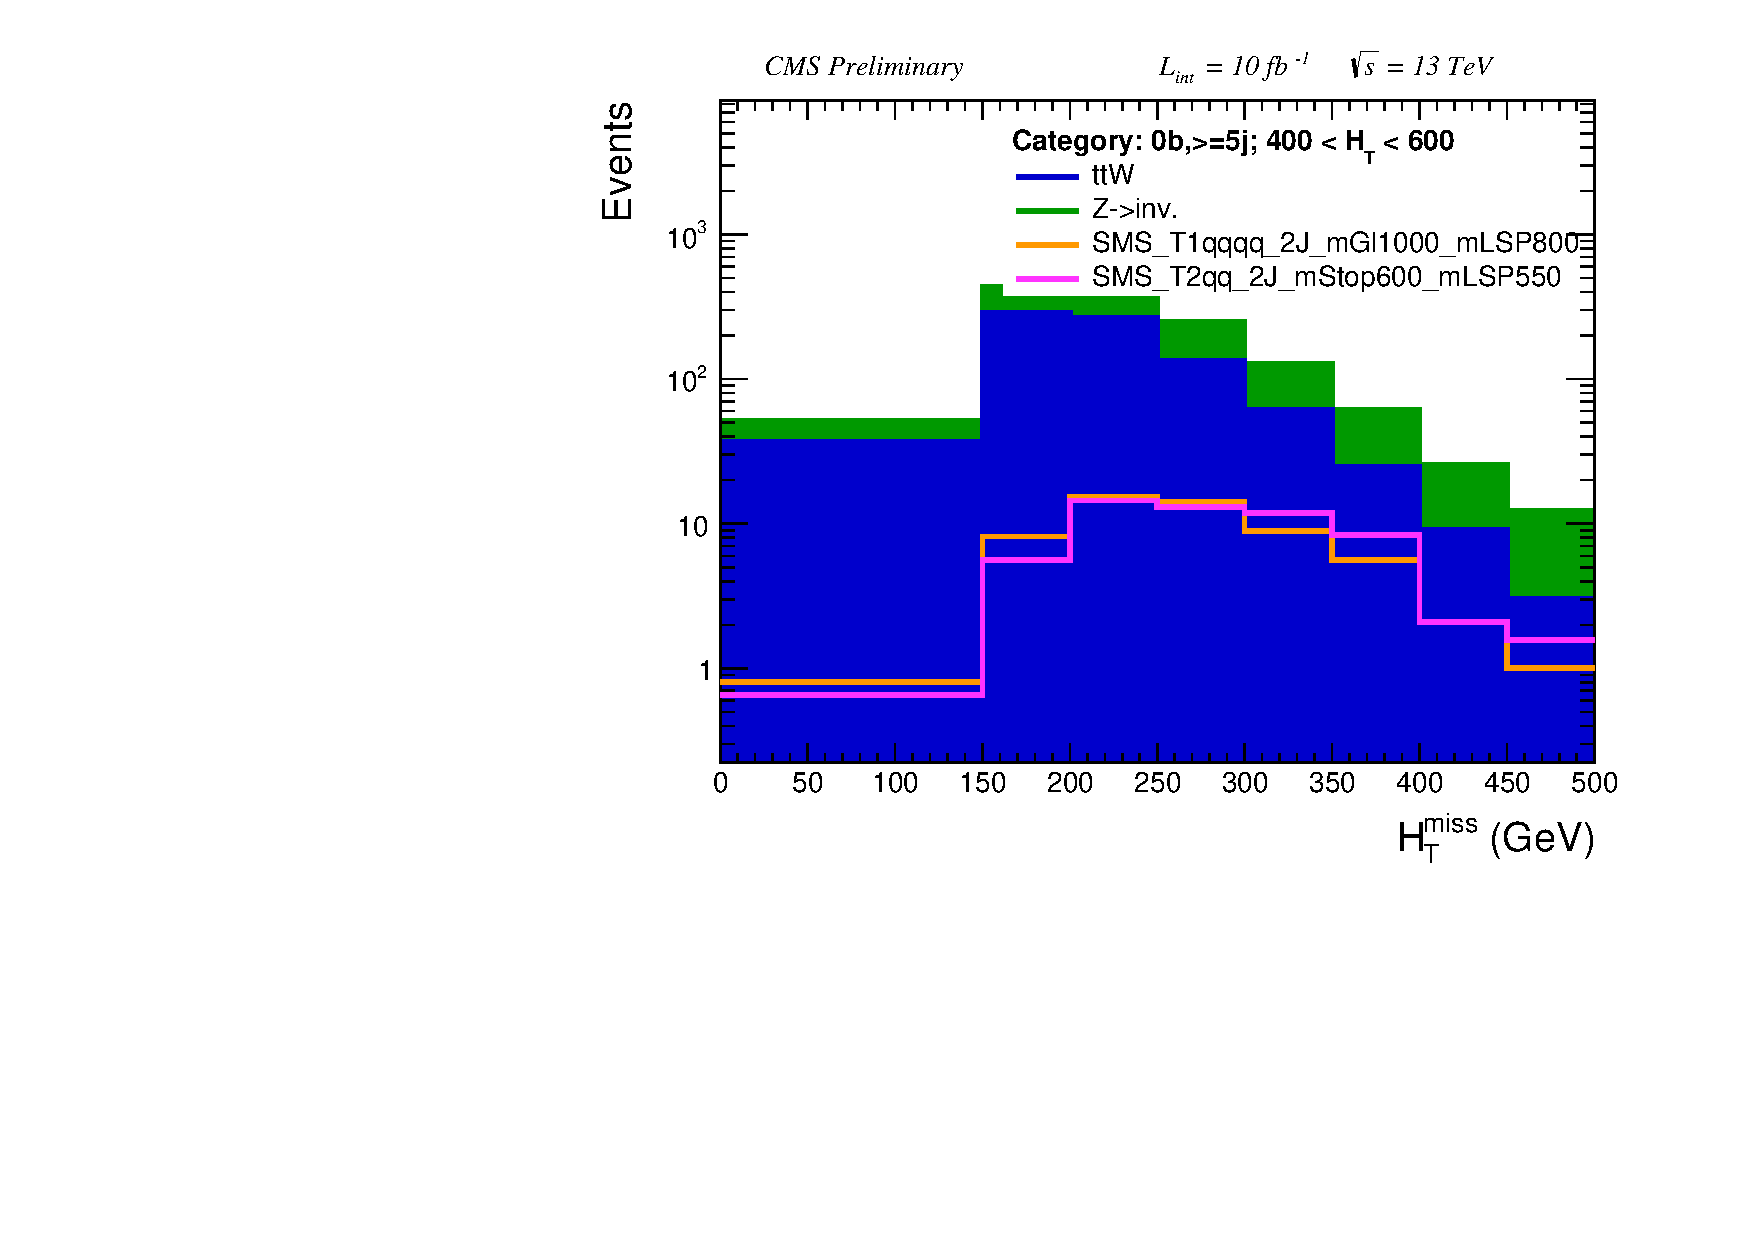
\includegraphics[width=0.5\textwidth]{figures/susyResults/MHT_eq0b_ge5j_400_600.pdf}} ~~
%%     \subfigure[$600 < \HT < 800  \gev$]{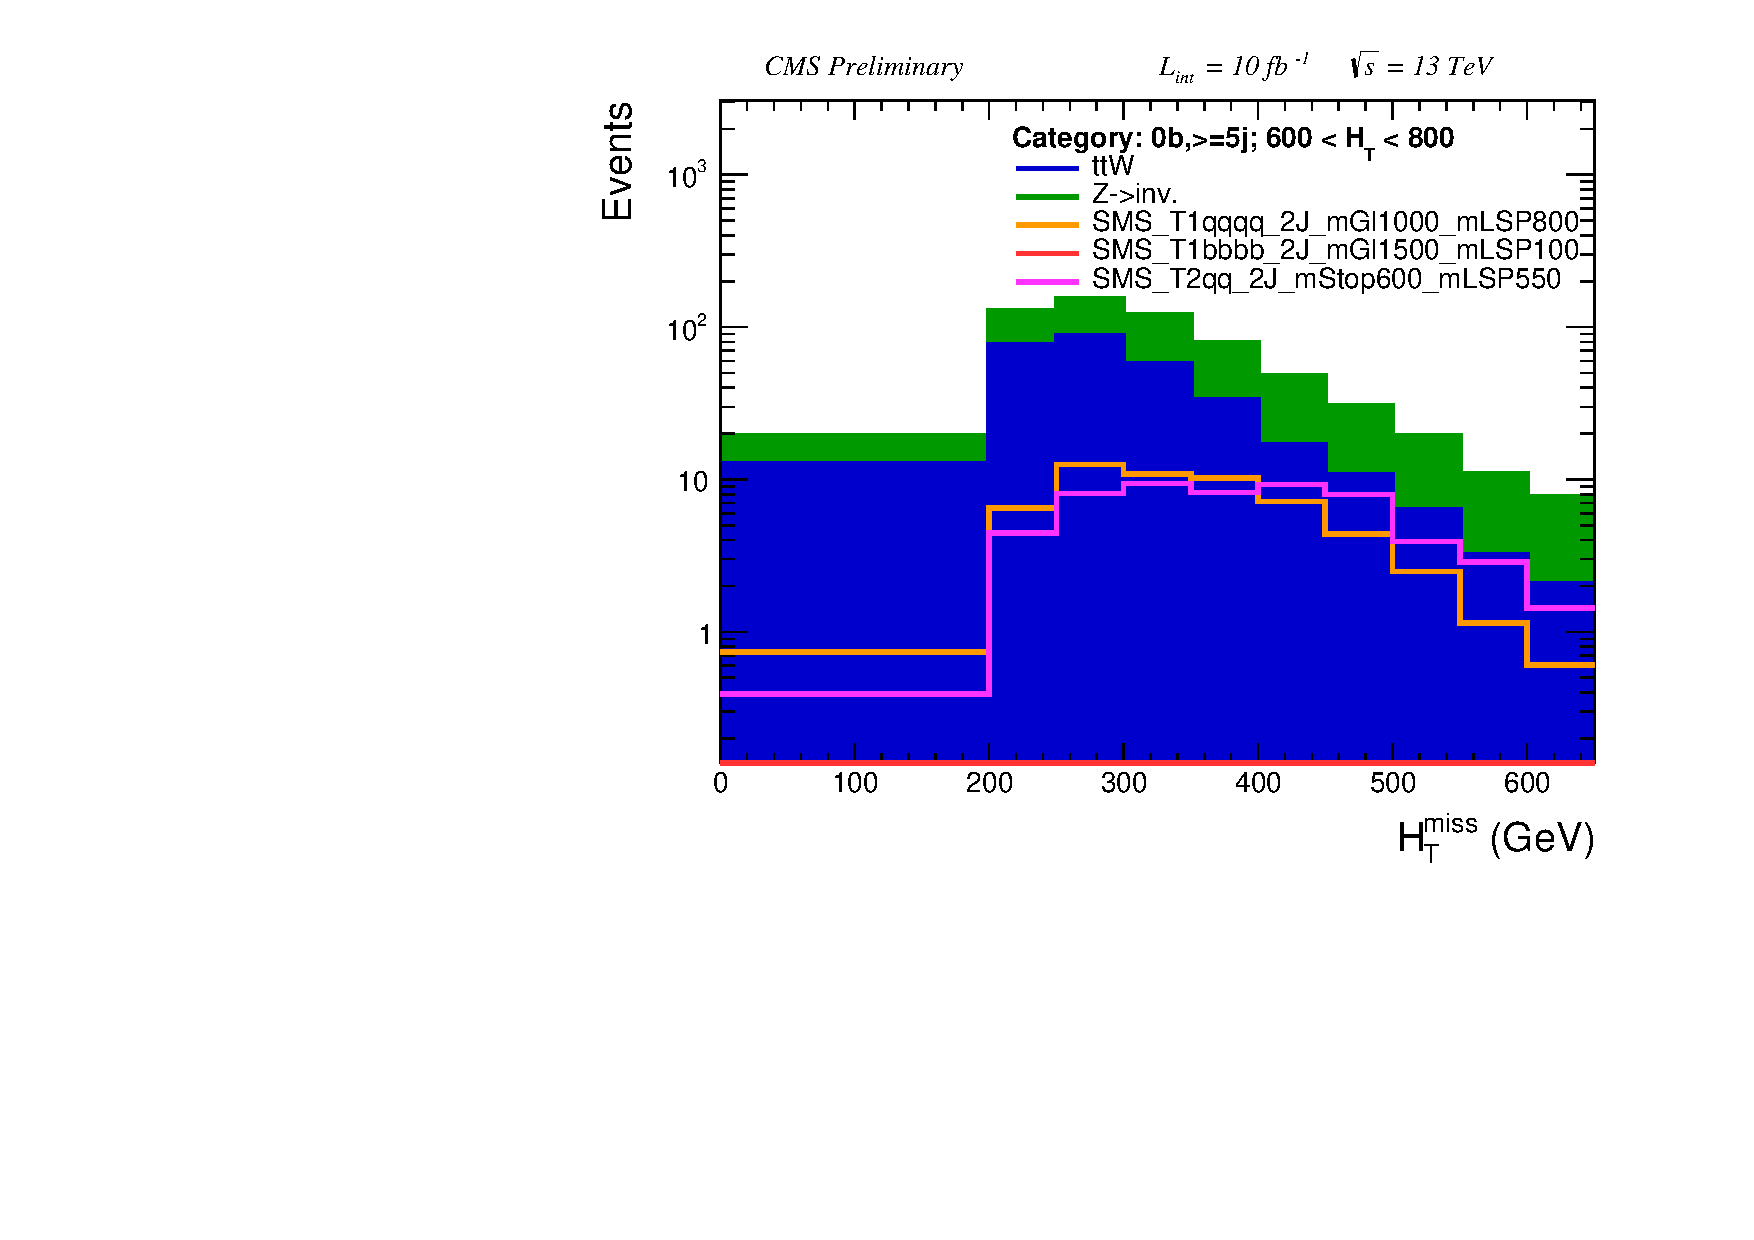
\includegraphics[width=0.5\textwidth]{figures/susyResults/MHT_eq0b_ge5j_600_800.pdf}} \\
%%     \subfigure[$\HT > 800 \gev$]{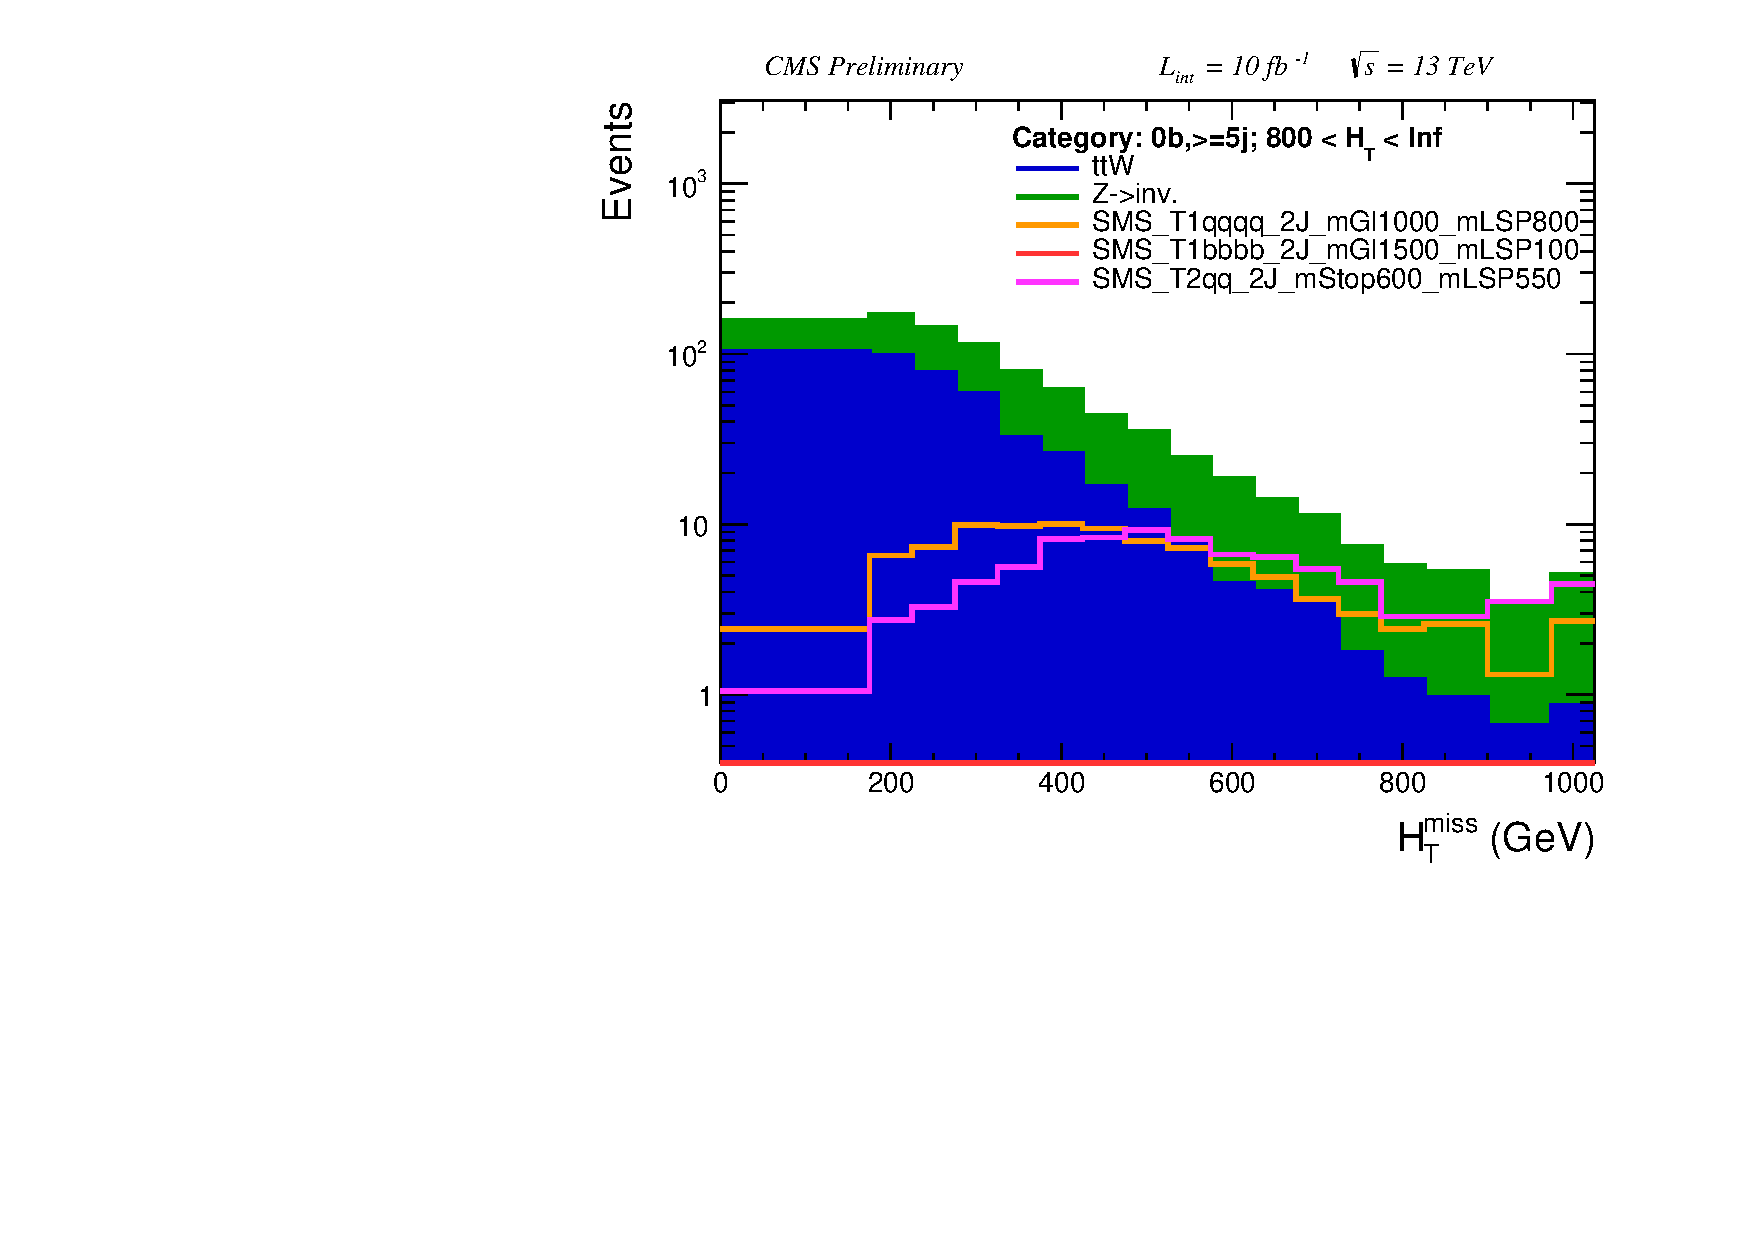
\includegraphics[width=0.5\textwidth]{figures/susyResults/MHT_eq0b_ge5j_800_Inf.pdf}}
%%     \caption{\mht templates for the $\njet\geq 5$, $\nb=0$ category.}
%%     \label{fig:mht_eq0b_ge5j}
%%   \end{center}
%% \end{figure}


%% \begin{figure}
%%   \begin{center}
%%     \subfigure[$350 < \HT < 400  \gev$]{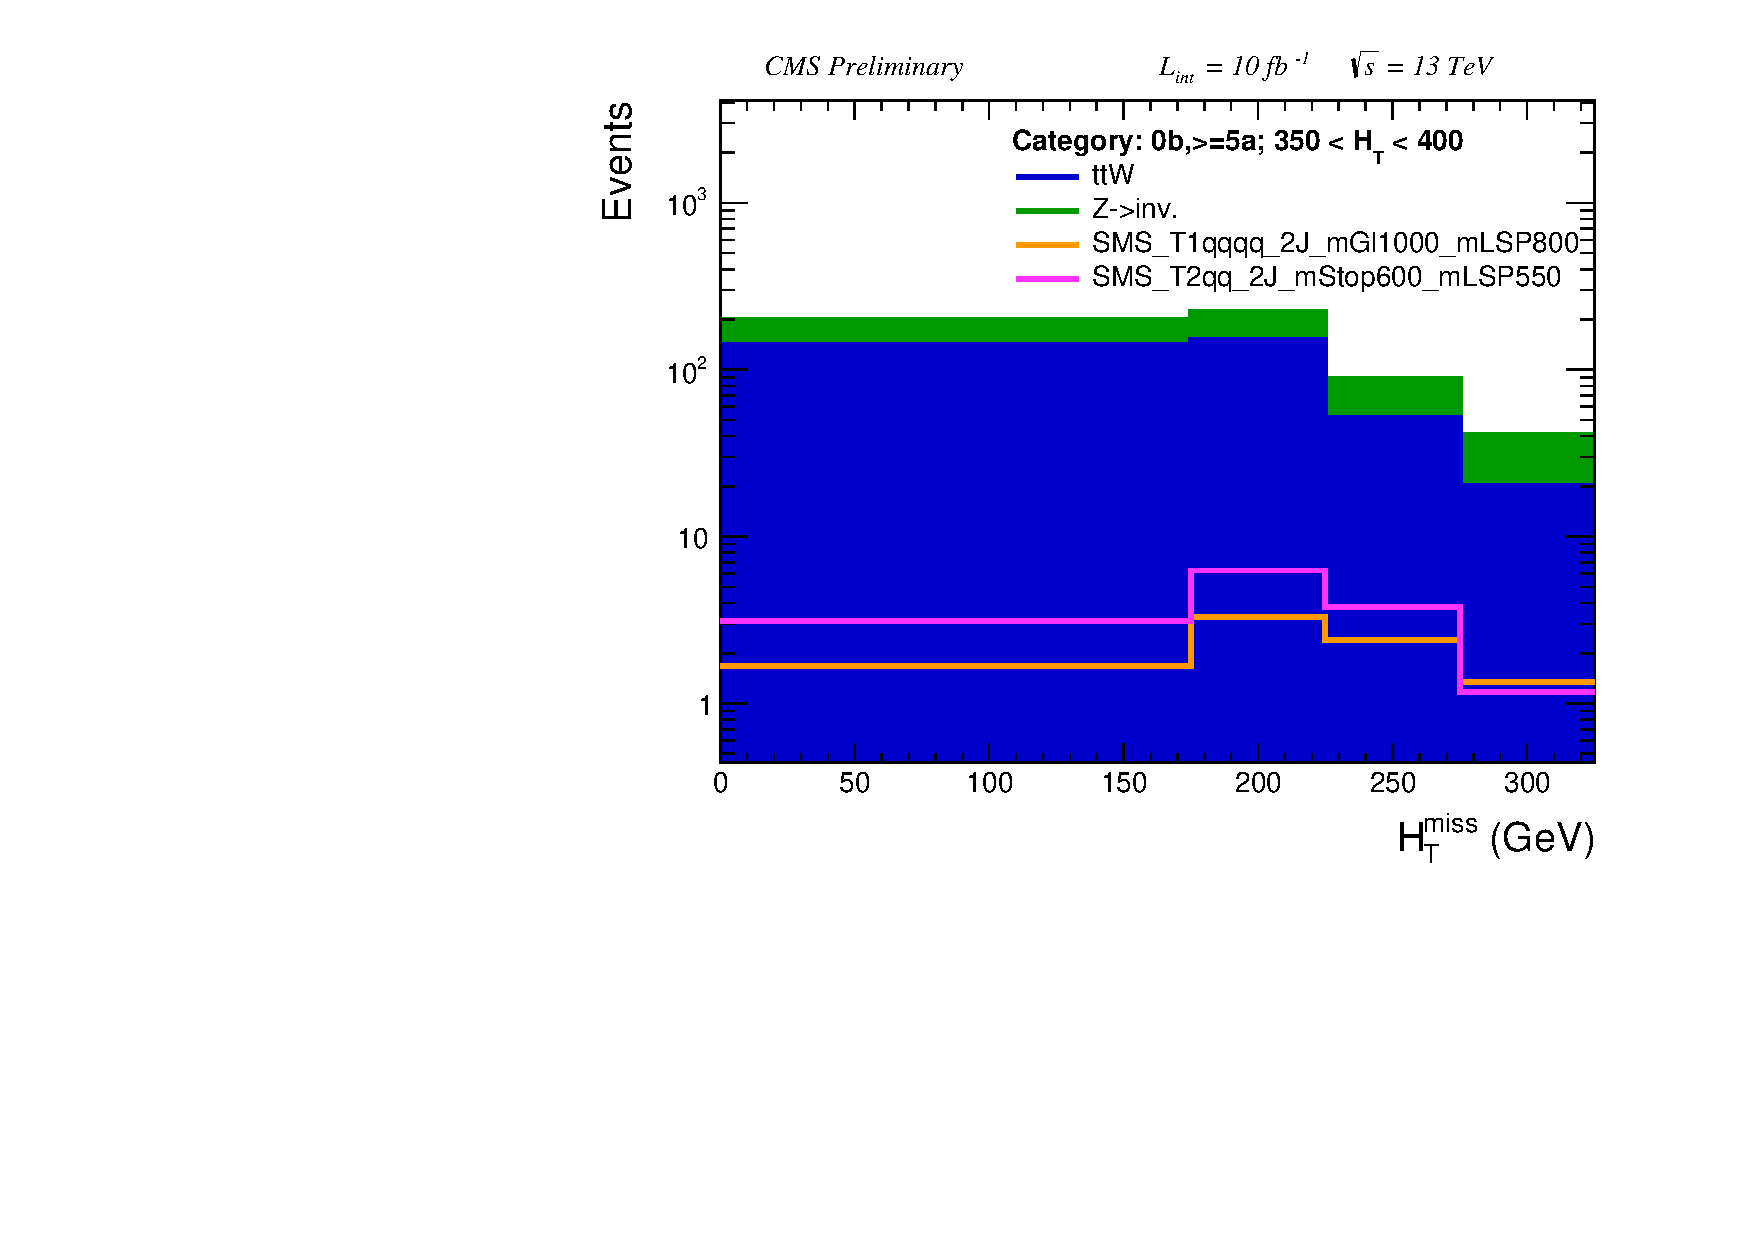
\includegraphics[width=0.5\textwidth]{figures/susyResults/MHT_eq0b_ge5a_350_400.pdf}} ~~
%%     \subfigure[$400 < \HT < 600  \gev$]{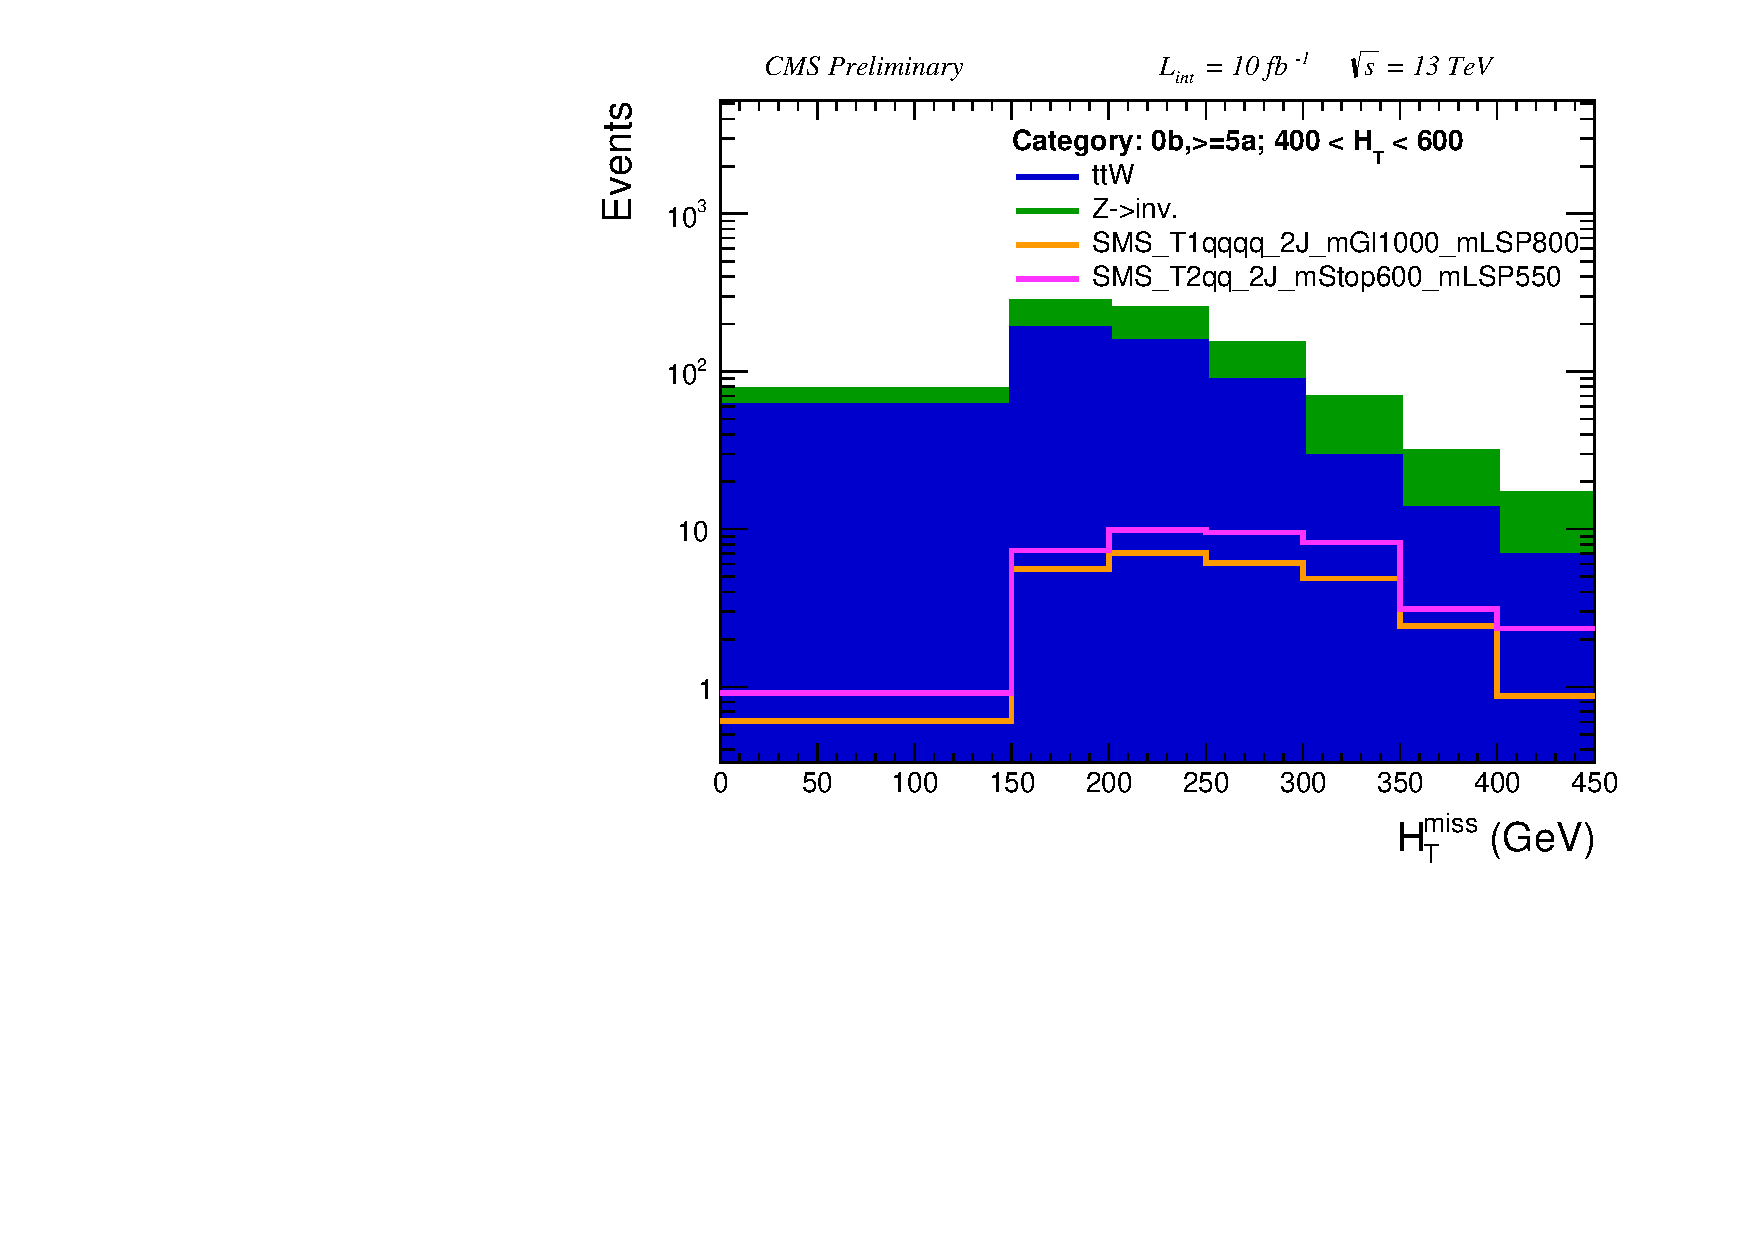
\includegraphics[width=0.5\textwidth]{figures/susyResults/MHT_eq0b_ge5a_400_600.pdf}}
%%     \caption{\mht templates for the $\njet\geq 5$ (asymmetric), $\nb=0$ category.}
%%     \label{fig:mht_eq0b_ge5a}
%%   \end{center}
%% \end{figure}


%% \begin{figure}
%%   \begin{center}
%%     \subfigure[$400 < \HT < 600  \gev$]{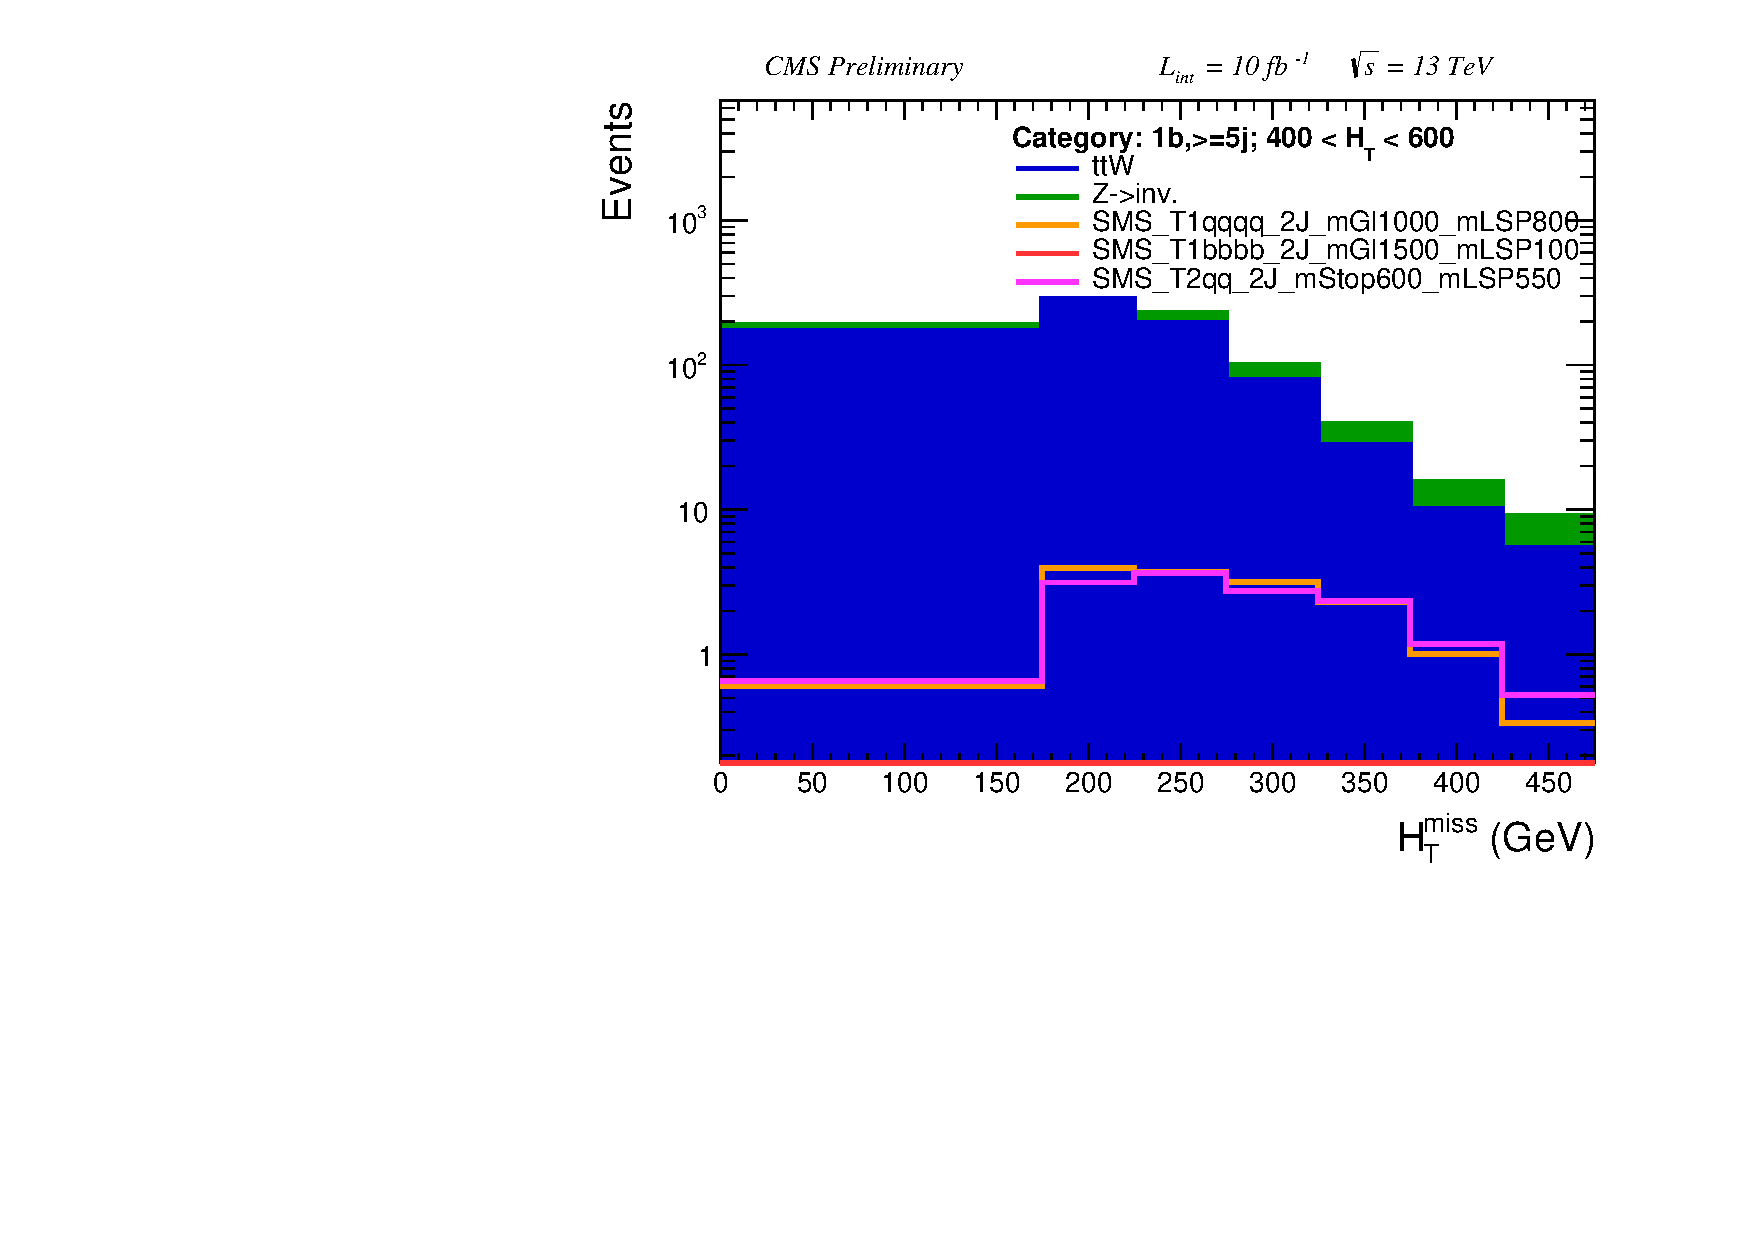
\includegraphics[width=0.5\textwidth]{figures/susyResults/MHT_eq1b_ge5j_400_600.pdf}} ~~
%%     \subfigure[$600 < \HT < 800  \gev$]{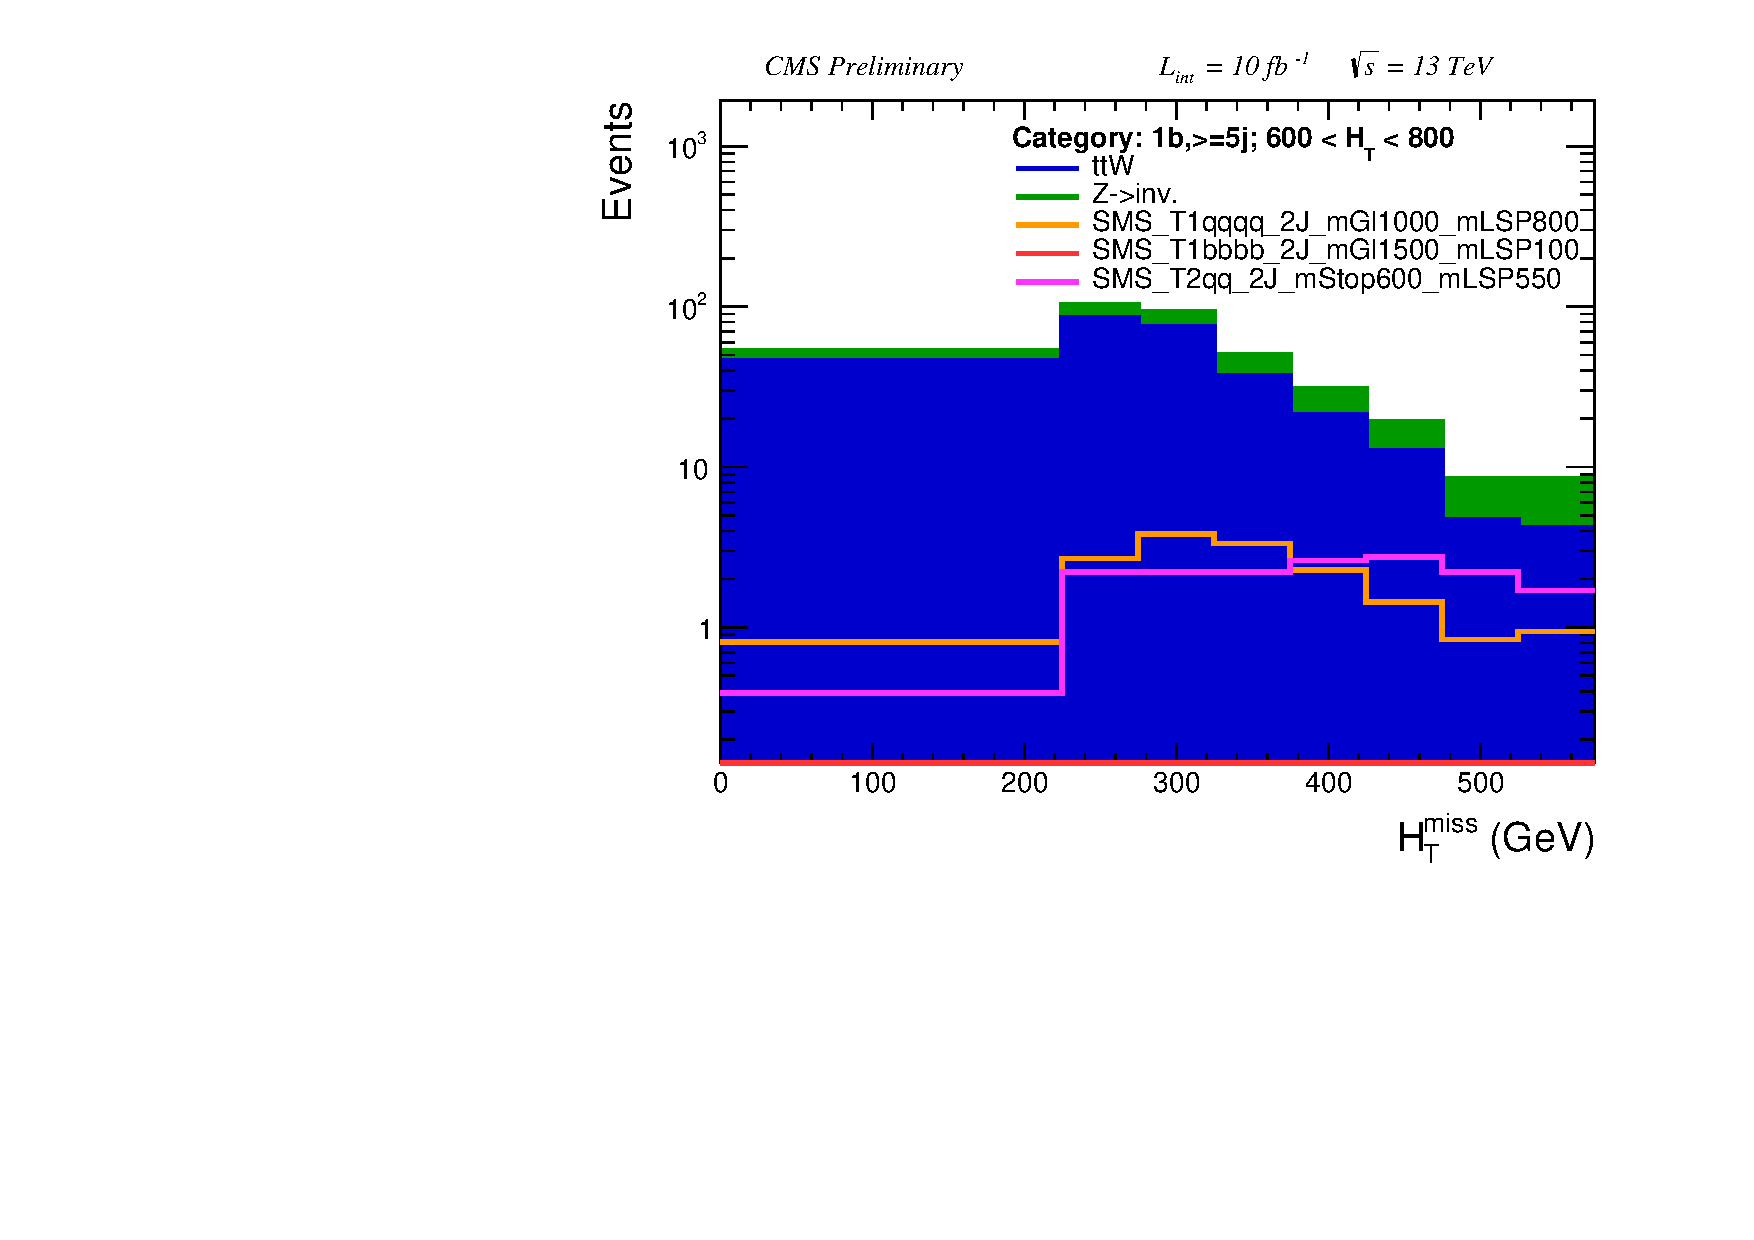
\includegraphics[width=0.5\textwidth]{figures/susyResults/MHT_eq1b_ge5j_600_800.pdf}} \\
%%     \subfigure[$\HT > 800 \gev$]{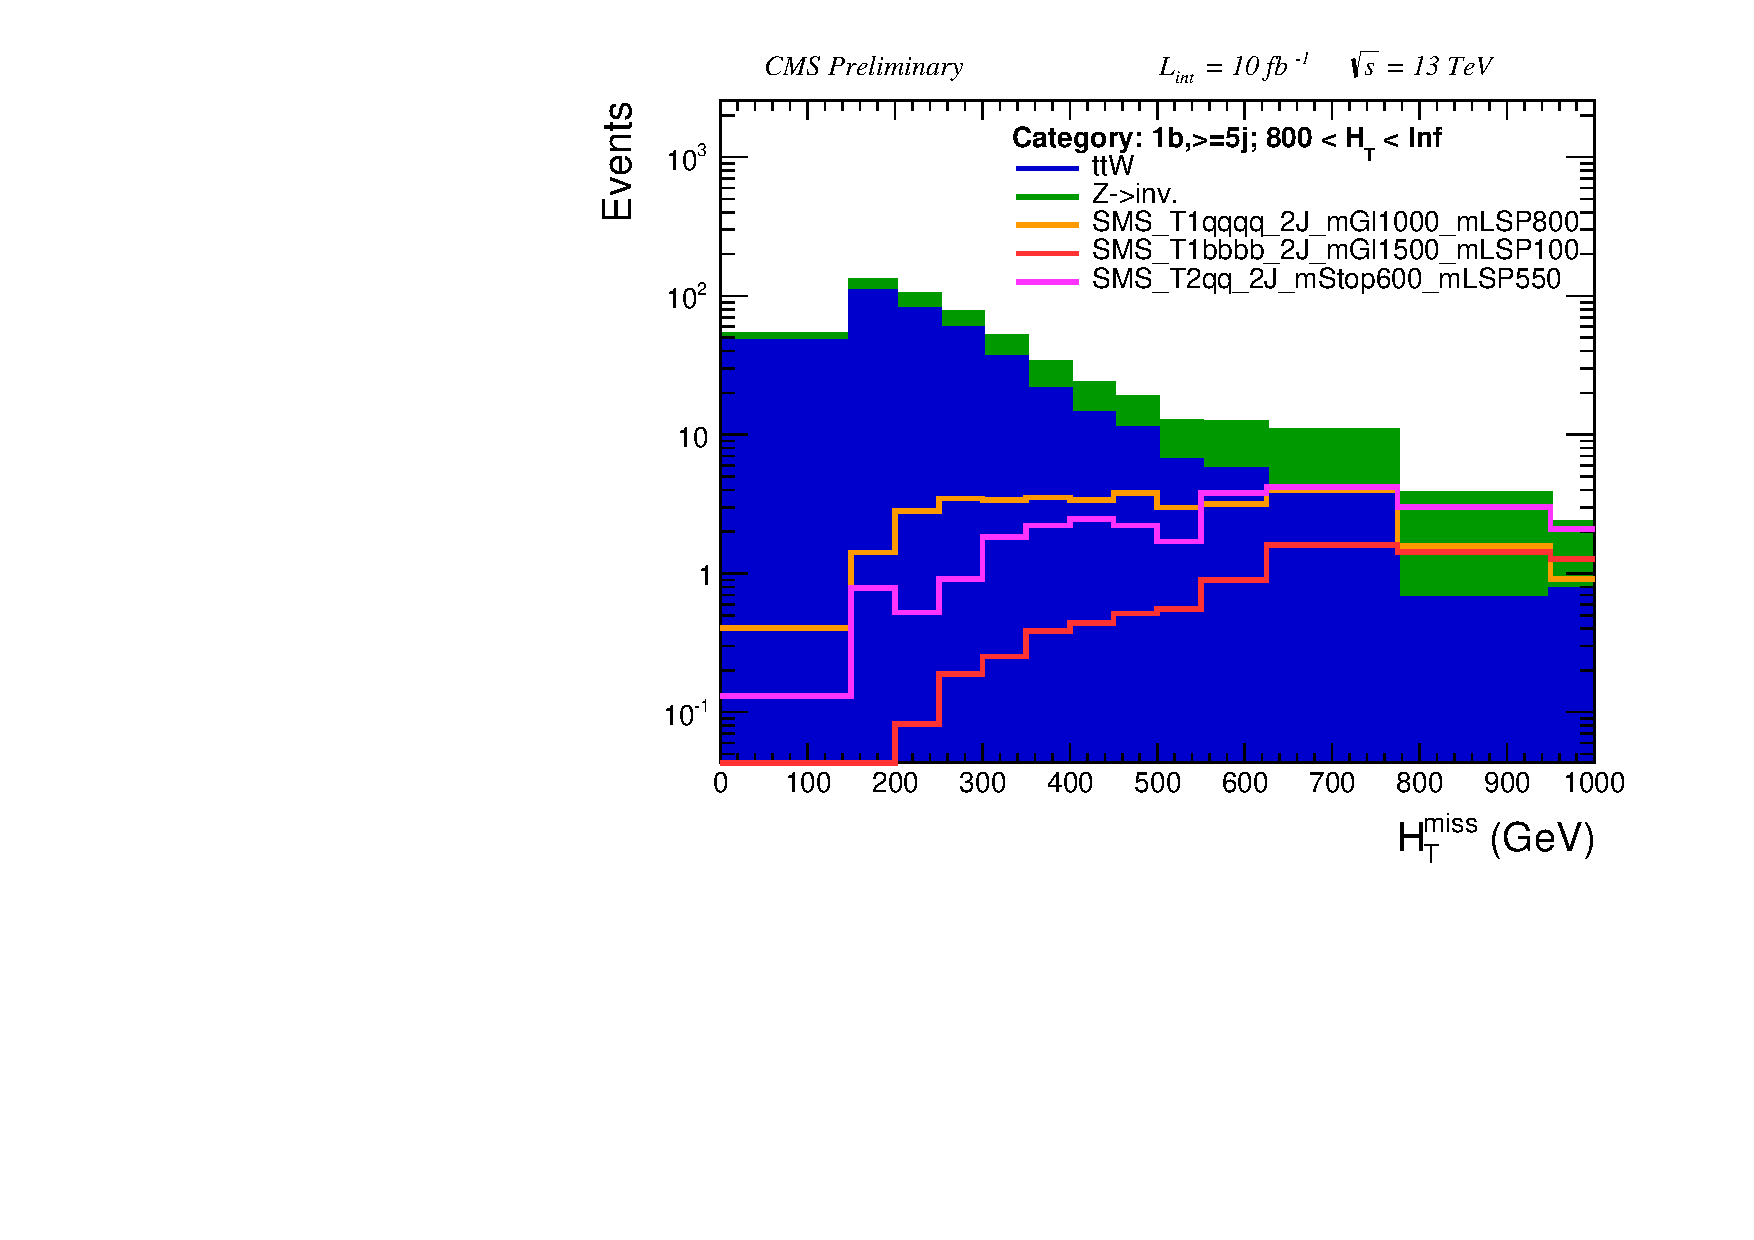
\includegraphics[width=0.5\textwidth]{figures/susyResults/MHT_eq1b_ge5j_800_Inf.pdf}}
%%     \caption{\mht templates for the $\njet\geq 5$, $\nb=1$ category.}
%%     \label{fig:mht_eq1b_ge5j}
%%   \end{center}
%% \end{figure}


%% \begin{figure}
%%   \begin{center}
%%     \subfigure[$350 < \HT < 400  \gev$]{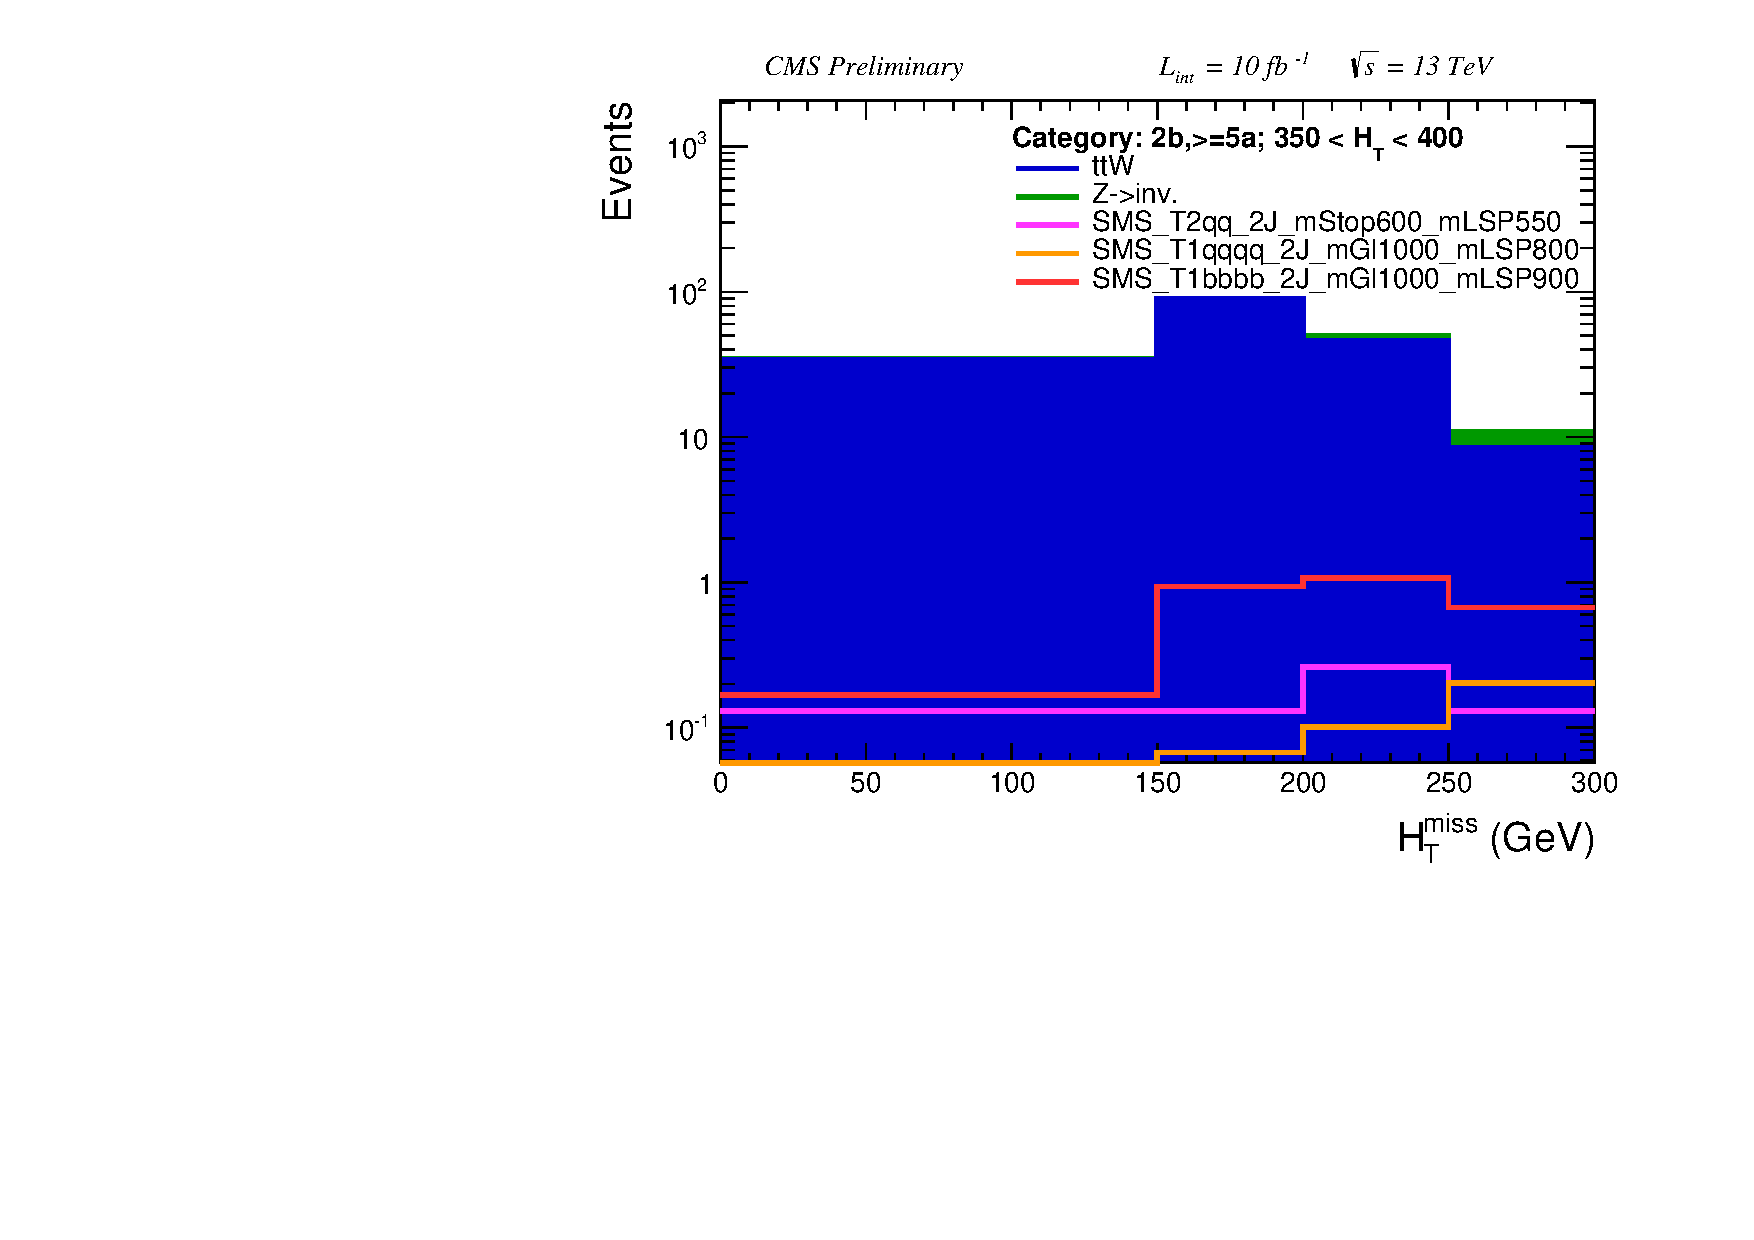
\includegraphics[width=0.5\textwidth]{figures/susyResults/MHT_eq2b_ge5a_350_400.pdf}} ~~
%%     \subfigure[$400 < \HT < 600  \gev$]{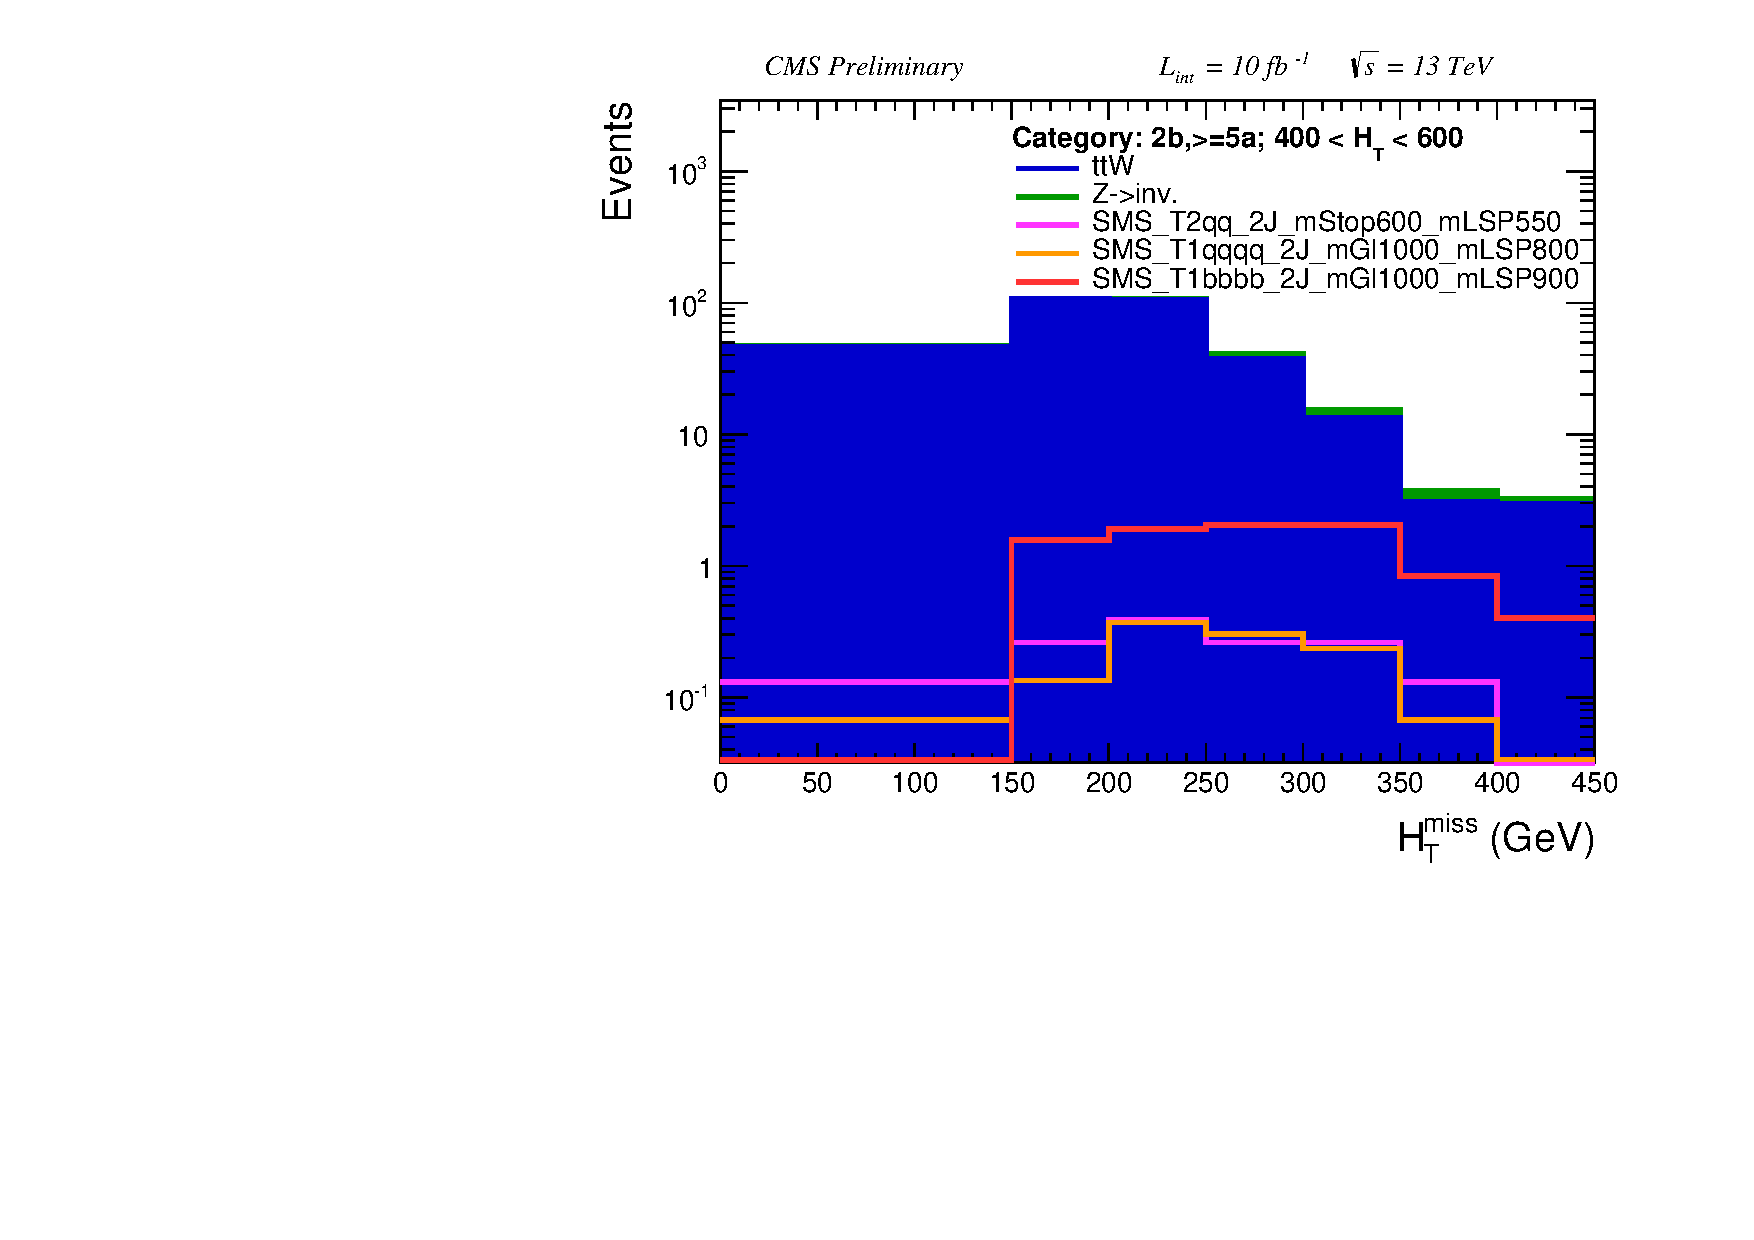
\includegraphics[width=0.5\textwidth]{figures/susyResults/MHT_eq2b_ge5a_400_600.pdf}} \\
%%     \subfigure[$600 < \HT < 800  \gev$]{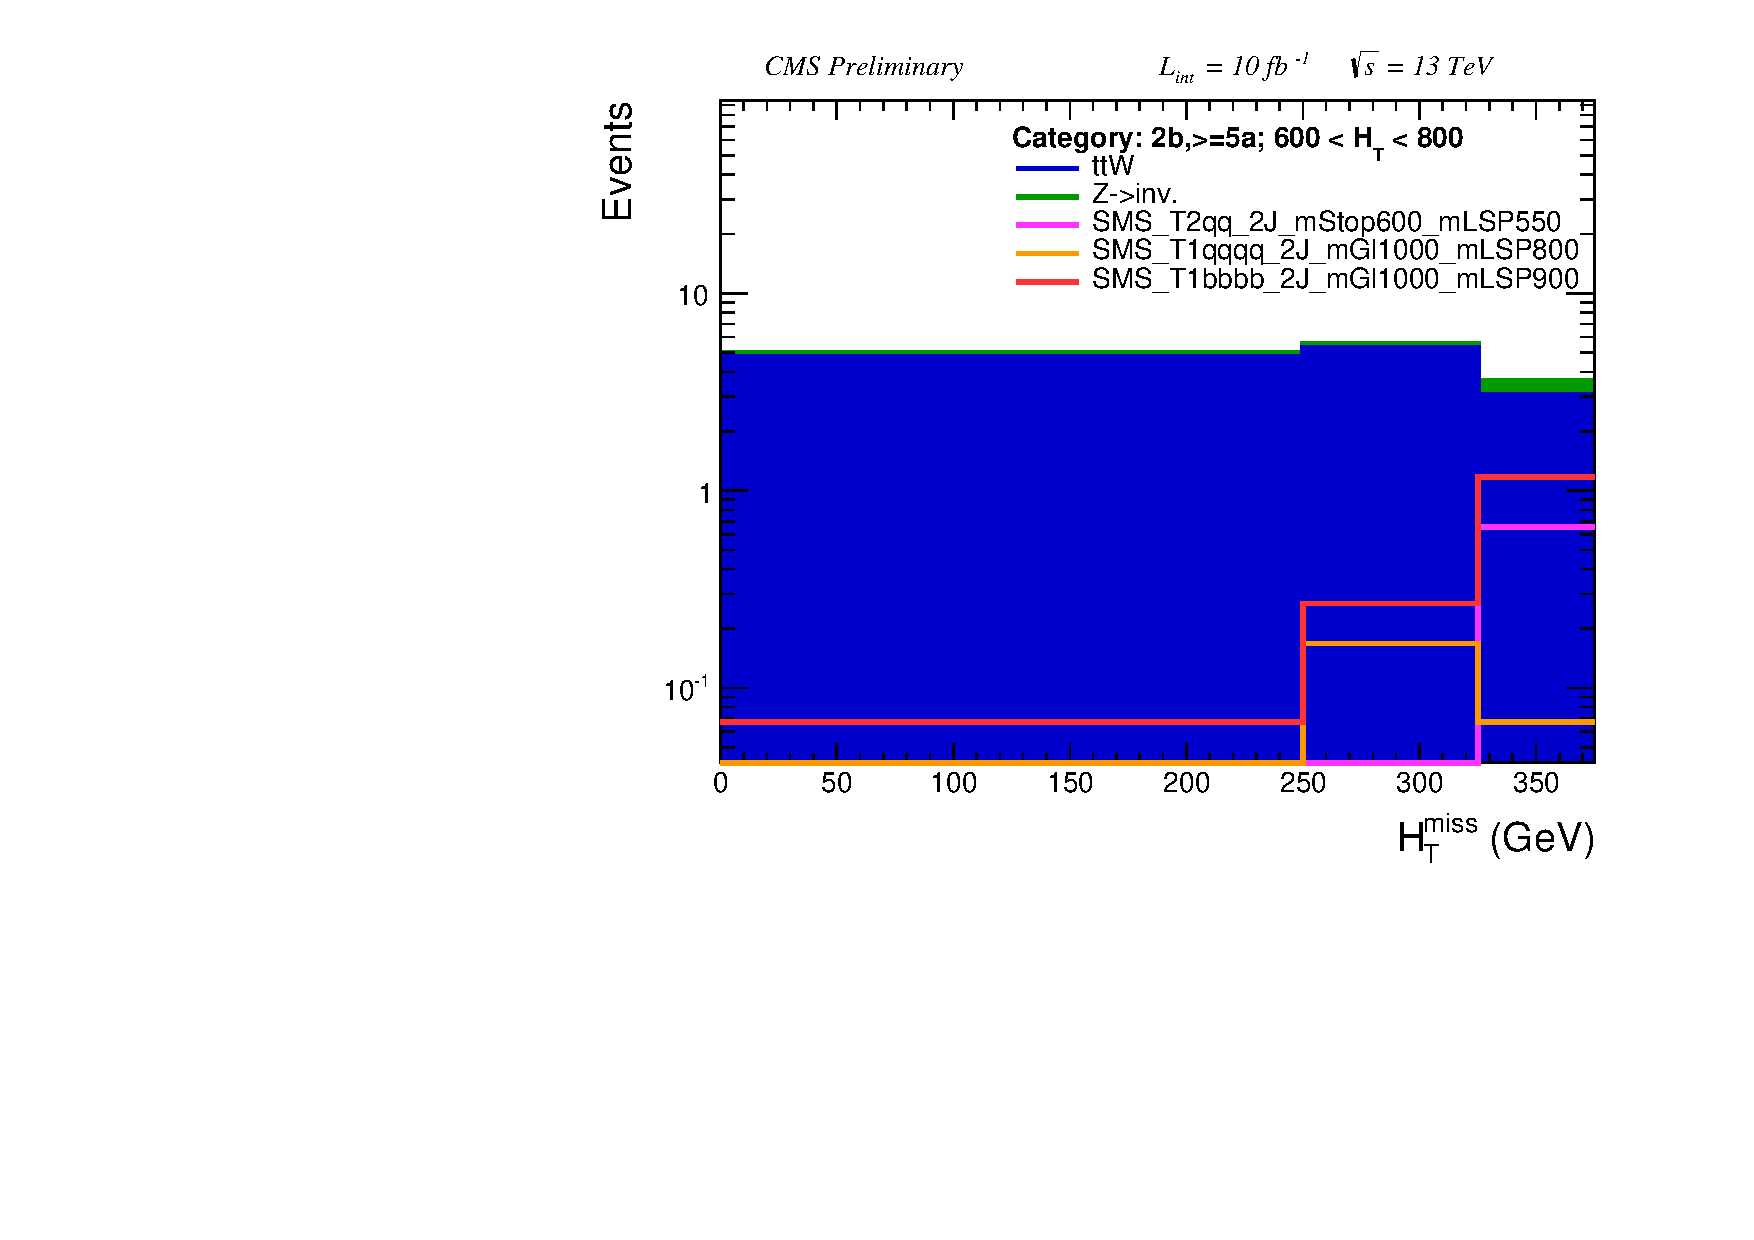
\includegraphics[width=0.5\textwidth]{figures/susyResults/MHT_eq2b_ge5a_600_800.pdf}} ~~
%%     \subfigure[$\HT > 800  \gev$]{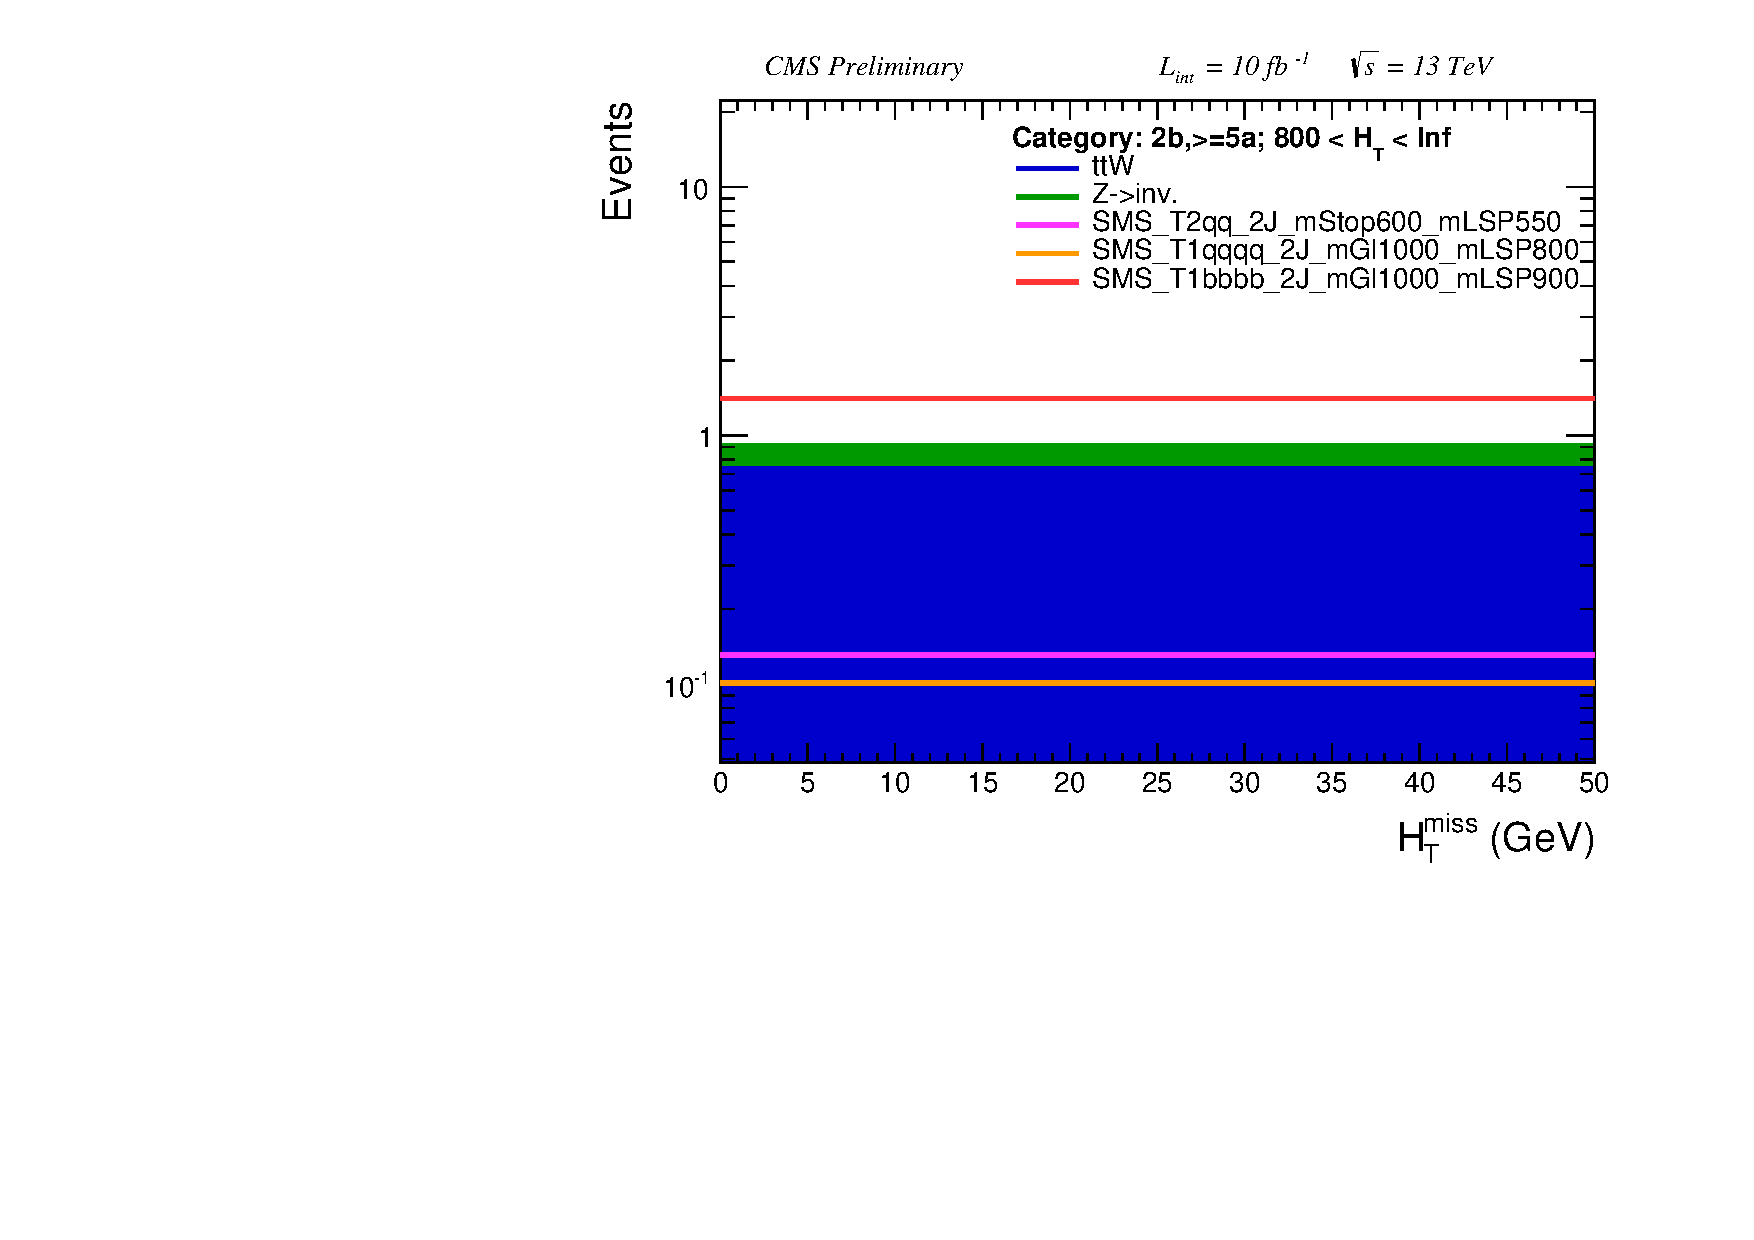
\includegraphics[width=0.5\textwidth]{figures/susyResults/MHT_eq2b_ge5a_800_Inf.pdf}} \\
%%     \caption{\mht templates for the $\njet=5$ (asymmetric), $\nb=2$ category.}
%%     \label{fig:mht_eq2b_ge5a}
%%   \end{center}
%% \end{figure}


%% \begin{figure}
%%   \begin{center}
%%     \subfigure[$400 < \HT < 600  \gev$]{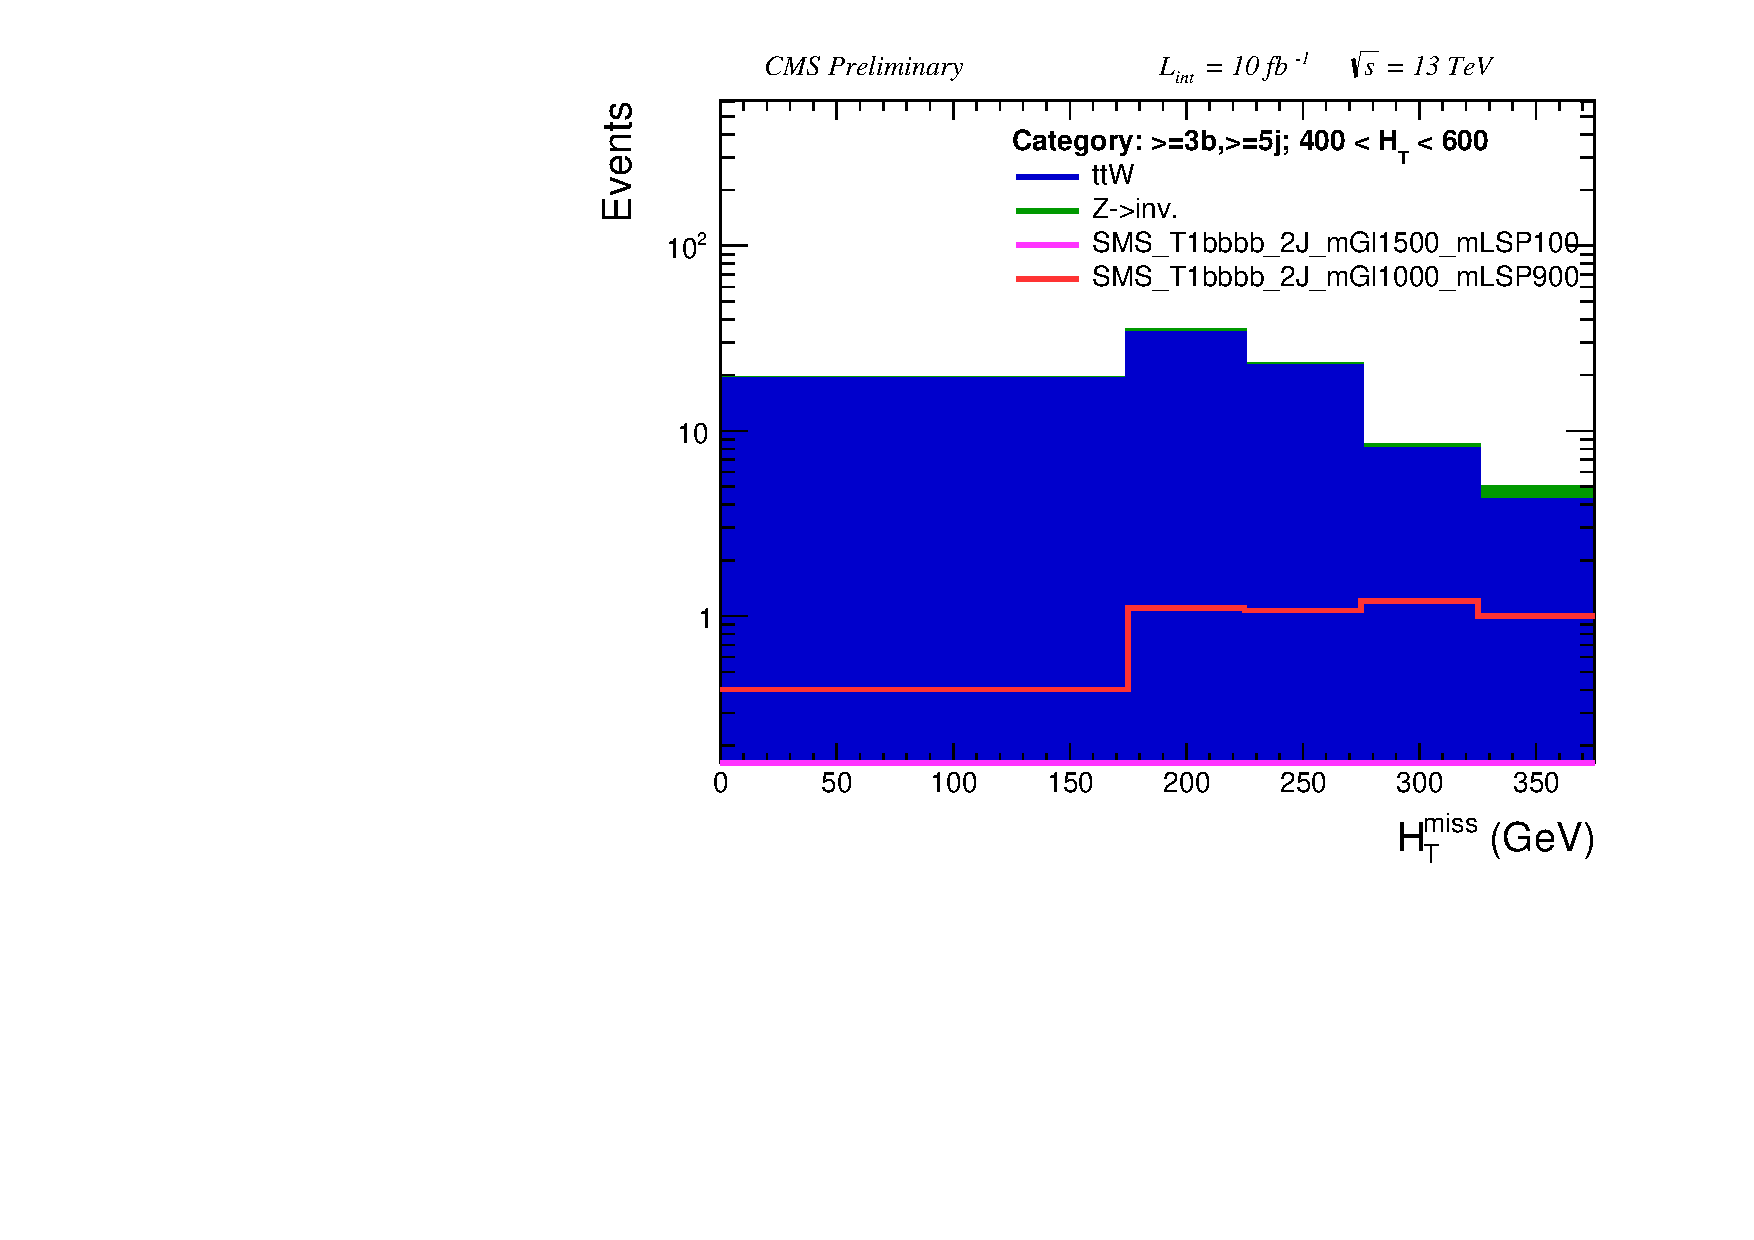
\includegraphics[width=0.5\textwidth]{figures/susyResults/MHT_ge3b_ge5j_400_600.pdf}} ~~
%%     \subfigure[$600 < \HT < 800  \gev$]{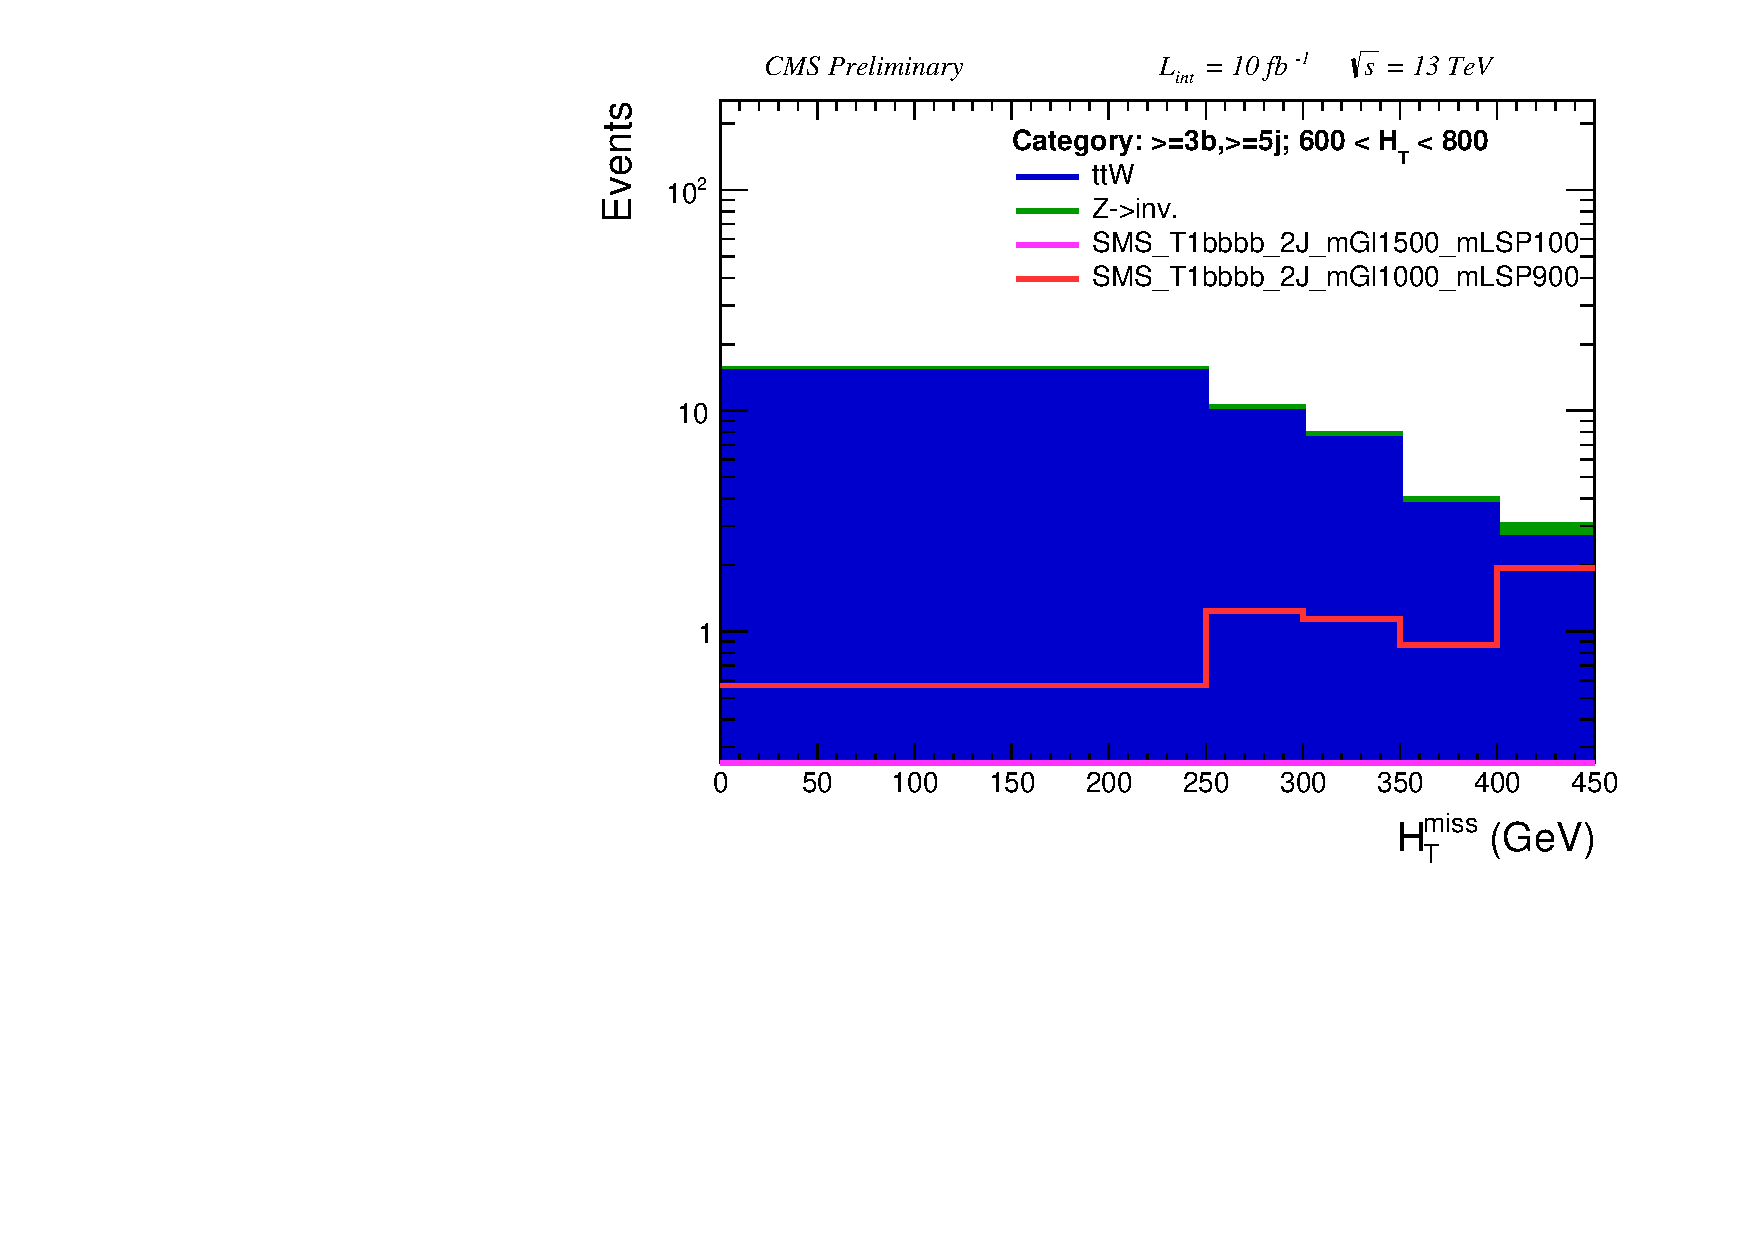
\includegraphics[width=0.5\textwidth]{figures/susyResults/MHT_ge3b_ge5j_600_800.pdf}} \\
%%     \subfigure[$\HT > 800 \gev$]{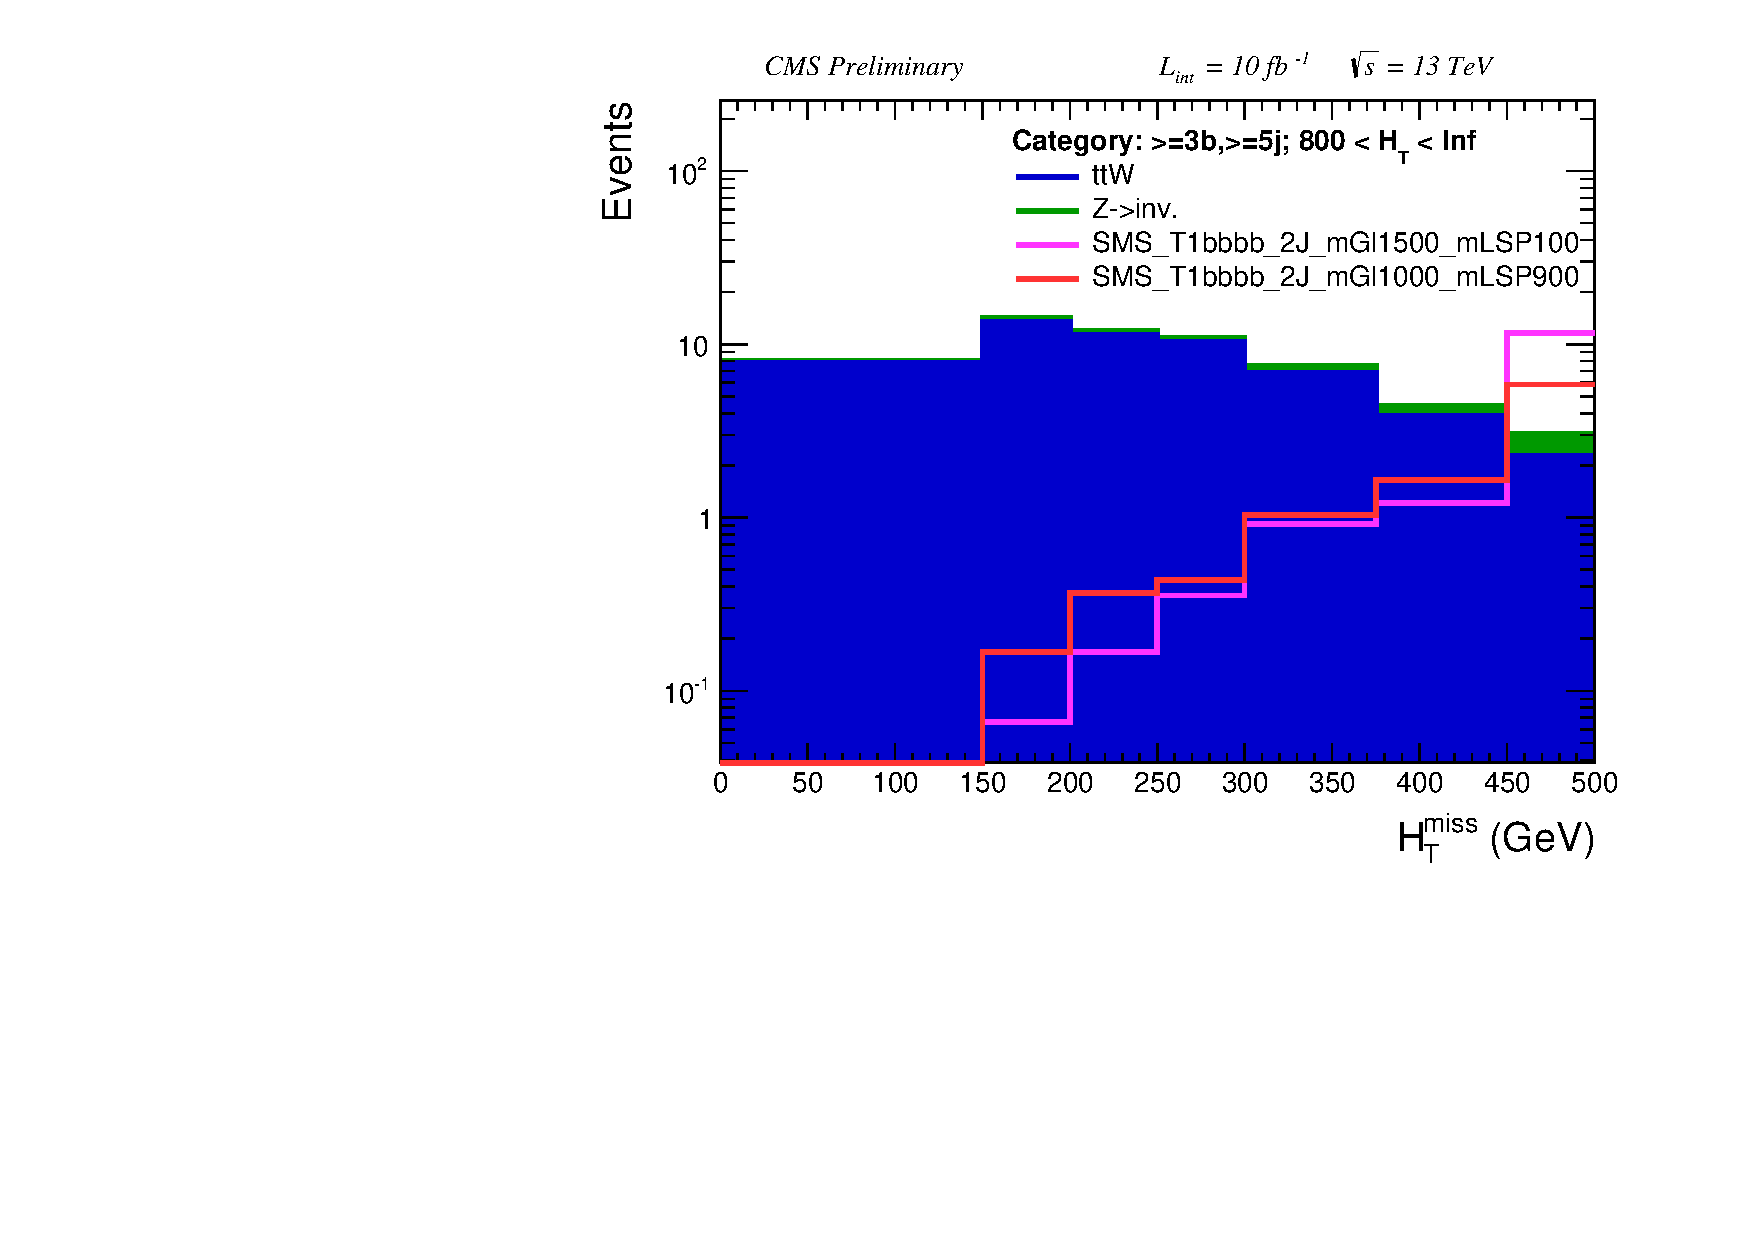
\includegraphics[width=0.5\textwidth]{figures/susyResults/MHT_ge3b_ge5j_800_Inf.pdf}}
%%     \caption{\mht templates for the $\njet\geq 5$, $\nb\geq 3$ category.}
%%     \label{fig:mht_ge3b_ge5j}
%%   \end{center}
%% \end{figure}


%% Tables~\ref{tab:results_ul} and \ref{tab:results_signif} show, respectively, 
%% the expected 95\% upper limit on the signal strength $\mu=\sigma/\sigma_{\mathrm{theory}}$ 
%% and the expected discovery significance, for all the simplified models. 
%% The projections are done for an integrated luminosity of 3 \ifb and 10 \ifb. 
%% The effect of including a ``toy'' template uncertainty (Sec.~\ref{sec:syst-on-shape}) is compared to the result without any template systematic.  

%% Both the significance and the limit are computed using the asymptotic formulae and the pre-fit Asimov datasets \cite{AsymptoticFormulae}. 
%% The upper limits are computed using the $\text{CL}_{s}$ criterion \cite{CLsTechnique}. \\
%% All the statistical results are produced using the \textit{combine} tool, 
%% provided within the HiggsAnalysis-CombinedLimit package \cite{Combine}. \\
%% For each model, the categories used in the combination are listed in Table \ref{tab:simplified-models}. 

%% \begin{table}
%%   \centering
%%   \caption{95\% C.L. upper limit on $\mu$ for the different benchmark models and the different luminosity scenarios. 
%%   The main result is obtained by applying 
%%   the ``toy'' template systematic described in Section~\ref{sec:syst-on-shape}, 
%% while in parentheses the result without any template systematic is reported. 
%% For T2qq, two degenerate light squark generations are assumed.}
%%   \label{tab:results_ul}
%%   \footnotesize
%%   \begin{tabular}{lcc}
%%     \hline
%%     \hline
%%     Signal model & $\mathcal{L} = 3 \ifb$ & $\mathcal{L} = 10 \ifb$ \\
%%     \hline
%%     \hline
%%     T1bbbb 1500,100  & 0.68 (0.66) & 0.33 (0.31) \\ 
%%     T1bbbb 1000,900  & 0.67 (0.62) & 0.35 (0.31) \\ 
%%     T1qqqq 1400,100  & 0.98 (0.82) & 0.54 (0.41) \\ 
%%     T1qqqq 1000,800  & 0.75 (0.65) & 0.42 (0.35) \\ 
%%     T1tttt 1500,100  & 1.9 (1.84) & 0.92 (0.86) \\  
%%     T1tttt 1200,800  & 3.89 (3.78) & 2.06 (1.93) \\ \hline
%%     T2tt 850,100     & 2.07 (1.91) & 1.13 (0.98) \\ 
%%     T2tt 650,325     & 2.3 (2.16) & 1.32 (1.18) \\  
%%     T2tt 500,325     & 3.48 (3.39) & 1.88 (1.79) \\ 
%%     T2tt 425,325     & 2.16 (2.02) & 1.19 (1.1) \\  
%%     T2qq 1200,100    & 1.75 (1.43) & 0.91 (0.7) \\  
%%     T2qq 600,550     & 0.57 (0.47) & 0.32 (0.24) \\ 
%%     T2bb 900,100     & 1.84 (1.71) & 0.92 (0.82) \\ 
%%     T2bb 600,580     & 4.89 (3.95) & 2.84 (2.13) \\ 
%%     \hline
%%     \hline
%%   \end{tabular} 
%% \end{table}


%% \begin{table}
%%   \centering
%%   \caption{Expected significance for the different benchmark models and the different luminosity scenarios. 
%%     The main result is obtained by applying 
%%   the ``toy'' template systematic described in Sec.~\ref{sec:syst-on-shape},
%% while in parentheses the result without any template systematic is reported. 
%% For T2qq, two degenerate light squark generations are assumed.}

%%   \label{tab:results_signif}
%%   \footnotesize
%%   \footnotesize
%%   \begin{tabular}{lcc}
%%     \hline
%%     \hline
%%     Signal model & $\mathcal{L} = 3 \ifb$ & $\mathcal{L} = 10 \ifb$ \\
%%     \hline
%%     \hline
%%     T1bbbb 1500,100  & 3.0 (3.3) & 5.2 (5.9) \\  
%%     T1bbbb 1000,900  & 3.0 (3.4) & 5.1 (6.2) \\  
%%     T1qqqq 1400,100  & 1.9 (2.6) & 3.2 (4.8) \\  
%%     T1qqqq 1000,800  & 2.6 (3.1) & 4.6 (5.6) \\  
%%     T1tttt 1500,100  & 1.3 (1.4) & 2.2 (2.5) \\  
%%     T1tttt 1200,800  & 0.6 (0.6) & 1.0 (1.1) \\  \hline
%%     T2tt 850,100     & 1.0 (1.2) & 1.8 (2.1) \\  
%%     T2tt 650,325     & 0.9 (1.0) & 1.5 (1.7) \\  
%%     T2tt 500,325     & 0.6 (0.6) & 1.1 (1.2) \\  
%%     T2tt 425,325     & 0.9 (1.0) & 1.7 (1.9) \\  
%%     T2qq 1200,100    & 1.1 (1.5) & 2.1 (2.9) \\  
%%     T2qq 600,550     & 3.3 (4.3) & 6.0 (8.0) \\  
%%     T2bb 900,100     & 1.2 (1.3) & 2.2 (2.5) \\
%%     T2bb 600,580     & 0.4 (0.5) & 0.7 (1.0) \\  
%%     \hline
%%     \hline
%%   \end{tabular} 
%% \end{table}


%%____________________________________________________________________________||
